\chapter{\texorpdfstring{\gls{co2}}{CO2} Sensing Using Fluorescent Thin Films}\label{chap:thin_film}

\begin{tldrbox}
	
	This chapter primarily contains chemical considerations about the practical implementation of an \gls{fdlr}, dye-based, thin film \gls{co2} sensor. In particular, the photobleaching and quenching issues generally plaguing luminescence measurements are briefly presented, along with strategies to mitigate their effect. Candidate dyes and polymers are then benchmarked to select the most suitable dye / polymer pairs for \gls{co2} sensing. The optoelectronics used to probe the manufactured thin films are also briefly presented. Finally, experimental results demonstrating accurate \invitro{} \gls{co2} sensing are reported. Photobleaching, quenching, and humidity cross-sensitivity are also studied, leaving open research avenues for the future.
	
	\tcblower
	
	\hyperref[chap:choosing_techno]{Previous chapter} \hfill \hyperref[chapter:toc]{Main Table Of Content (TOC)} \hfill \hyperref[chap:conclusion]{Next chapter}
	
\end{tldrbox}

While the previous chapters of this doctoral work are mainly focused on
\begin{enumerate}
	\item the motivations behind transcutaneous \gls{co2} sensing (Chapter \ref{chap:intro}),
	\item the feasibility of the latter given the properties of
	\begin{enumerate}[label=(\alph*)]
		\item haemoglobin (Chapter \ref{chap:co2hb}) and
		\item skin \gls{co2} exhalation (Chapter \ref{chap:tcco2}),
	\end{enumerate}
	\item the choice of a given \gls{co2} measurement technique, and
	\item the theoretical developments surrounding its implementation (Chapter \ref{chap:choosing_techno}),
\end{enumerate}
the present chapter focuses on the practical implementation of the said technique into a fully functional sensor. More specifically, the pH-sensitive and reference luminophores need to be dispersed and immobilised into a polymer matrix, which should ideally maintain satisfying humidity levels while limiting the photobleaching of the luminophores.

Section \ref{sect:thin_film:encaps} thus discusses different encapsulation strategies, presenting the photobleaching and quenching phenomena, as well as the deleterious influence of \gls{o2} on the latter. Sections \ref{sect:thin_film:select_lumino} and \ref{sect:thin_film:select_poly} are then dedicated to the choice of the two luminophores and polymers that will be used in the final sensors, respectively. Subsequently, Section \ref{sect:thin_film:opto_elec} presents briefly the optoelectronics that were used to probe the luminescent sensing films, while the complete design study of the optical setup is relegated to Appendix~\ref{app:optical_design}. Finally, Section \ref{sect:thin_film:results} showcases the actual realisation of \gls{co2}-sensing thin films using the above-mentioned luminophores, polymers, and optoelectronics. Basic sensing properties are demonstrated, some theoretical predictions are validated experimentally, and several caveats are also briefly exposed, opening new research avenues that are detailed in the next---and final---chapter. Of note, the impatient reader interested only in a minimalist summary of these practical works might be interested in reading our short---four pages---2024 NEWCAS article entitled \textit{Dual Lifetime Referencing for Accurate \gls{co2} Sensing: An Experimental \textit{in vitro} Validation}\cite{dervieux2024newcas}.

\section{Encapsulation Strategies}\label{sect:thin_film:encaps}

As mentioned in Section~\ref{sect:choos:dye_based:optical_schemes}---and contrary to \gls{fret}---\gls{fdlr} does not require both luminophores to be in close contact with each other. This is fortunate, since both luminophores call for very different encapsulations: while the pH-sensitive fluorophore needs a strongly hygroscopic medium with a good \gls{co2} permeability---see Section \ref{subsect:thin_film:breath_poly}---the reference phosphor needs a gas-tight encapsulation to prevent its exposure to \gls{o2}, which would likely worsen its photobleaching. Section \ref{subsect:thin_film:encaps:photobleaching} details the latter issue, while Section \ref{subsect:thin_film:encaps:strategies} presents resulting encapsulation strategies.

\subsection{Photobleaching and \texorpdfstring{\gls{o2}}{O2} Influence}\label{subsect:thin_film:encaps:photobleaching}

Not to be confused with the luminescence \emph{decay} phenomenon---which is defined as the decreasing luminescence intensity following a pulsed illumination, and characterised by a luminescence lifetime $\tau$, as mentioned in Section \ref{subsect:choos:dye_based:optical_schemes:dlr_intro}---the \emph{photobleaching} phenomenon---\aka{} photoinduced or photochemical degradation, fading, or photodegradation---corresponds to the irreversible destruction of luminophore molecules under illumination. This fundamental difference is illustrated in Figure~\ref{fig:thin_film:pbl:pbl_principle}, Left.

\begin{figure}
	\centering
	\includegraphics{1_main_matter/thin_film_figures/encasp_pbl/tikz/out/pbl_principle.pdf}
	\caption[Difference between luminescence decay and photobleaching, and possible photobleaching pathways.]{\textbf{Left:} difference between photobleaching and luminescence decay. In green is the luminescence intensity of a luminophore excited by a train of pulses. Each pulse causes a reproducible luminescence decay of lifetime $\tau$ (considering a mono-exponential decay, which is not necessarily the most accurate model, although being widely spread\cite{wlodarczyk2003}). Meanwhile, the repetition of pulses progressively destroys dye molecules, causing a slow but irreversible decrease in overall luminescence intensity: photobleaching is observed. Adapted from Song \etal{}\cite{song1995}. \textbf{Right:} simplified Perrin-Jablonski diagram of a luminophore, illustrating single and multiple photon absorption, non radiative decays (NRD), intersystem crossing (ISC), fluorescence, phosphorescence, and possible photobleaching pathways. See the text for further explanations. Elaborated from Demchenko\cite{demchenko2020} and Valeur\cite[Chap.~3]{valeur2012molecfluo}.}
	\label{fig:thin_film:pbl:pbl_principle}
\end{figure}

Photobleaching has been a long known phenomenon, but---despite intense research efforts---its intricacies remain relatively obscure, even by the admission of recently published reviews on the topic\cite{zheng2017pbl, demchenko2020}. While a thorough discussion on photobleaching is beyond the scope of this thesis, the curious reader may refer to the works of Diaspro \etal{}\cite{diaspro2006}, Zheng \etal{}\cite{zheng2017pbl} and Demchenko\cite{demchenko2020}, which, taken together, constitute an excellent introduction that covers the main aspects of the subject. Briefly, photobleaching describes photoinduced chemical reactions that lead to the conversion of the luminescent molecule into a by-product which is non-luminescent, hence decreasing the overall luminescence intensity of a given sample with time and illumination intensity. The photoinduced part comes from the fact that excited singlet or triplet states tend to be more chemically reactive than the basal S$_0$ state\footnote{If the reader is not familiar with Perrin-Jablonski diagrams nor the notion of singlet / triplet states, they might refer to the first three chapters of Bernard Valeur's \textit{Molecular Fluorescence}\cite{valeur2012molecfluo}.}, leading to photobleaching pathways alike those depicted in Figure~\ref{fig:thin_film:pbl:pbl_principle}, Right. While \gls{o2} and other \gls{ros} are often cited as being the main culprits for photobleaching, their deleterious influence seems to be especially significant for the T$_1$ photobleaching pathway, and other pathways may originate from dye-dye, or dye-solvent reactions taking the S$_1$ photobleaching pathway, for instance\cite{hinkeldey2008}.

The main difficulty in studying the photobleaching phenomenon comes from the fact that every dye is subjected to different photobleaching mechanisms, which also depend on:
\begin{enumerate}
	\item its concentration, with higher concentrations favouring dye-dye interactions\cite{song1997},
	\item the illumination intensity, with higher intensities favouring multiple photon absorption and thus excitation to higher S$_\text{n}$ states and subsequent photobleaching from there\cite{widengren1996},
	\item its surrounding medium, with marked differences between in-solution and \invitro{} photobleaching behaviours\cite{widengren1996},
	\item the solvent used\cite{woodford2017}.
\end{enumerate}
As a result, accurate photobleaching pathways are known only for a limited number of intensively studied luminophores---\eg{} erythrosine, as well as various fluorescein, rhodamine, and coumarin derivatives\cite{zheng2017pbl, song1995, karlsson2017}---and remain to be brought into light for the vast majority of luminophores.

Despite exhibiting some degree of usefulness in characterising the transport of luminescent molecules in cells\cite{axelrod1976}, photobleaching is more often than not considered to be a bane plaguing luminescence measurements, and its existence alone fully justifies the development of the ratiometric technique presented in Section~\ref{subsect:choos:dye_based:optical_schemes:ratiometric} to mitigate dye concentration decrease with time. More generally, fighting against photobleaching is no easy task, since the means for combatting it must be adapted to the photobleaching pathways involved. For instance, higher order S$_\text{n}$ pathways may be avoided by keeping the illumination power low, thereby limiting multiple photon absorption\cite{widengren1996, diaspro2006}. Targeting the same objective, using multiple low-intensity pulses instead of rarer high-intensity ones also results in less photobleaching\cite{donnert2007, ji2008}. Molecular engineering is another trail to follow to derive more stable compounds from already-known luminophores\cite{sun1997}, and lowering dye concentration may also reduce photobleaching rate\cite{song1997}. Then, so-called anti-fading agents may be added, which have different modes of operation: they may prevent either oxidation or reduction of the dyes following their ionisation in S$_\text{n}$ states, or quench their long-lived triplet state to favour a quick return to S$_0$ and thereby decrease the probability of a dye molecule to react with singlet oxygen or other \gls{ros}\cite{diaspro2006}. Finally, removing oxygen or \gls{ros} from the medium is one obvious solution since it often greatly reduces photobleaching, especially if the latter originates from long-lived triplet states\cite{song1995, widengren1996}.

In this thesis, I solely focused on this last aspect, leaving the use of anti-fading agents as a potential avenue for future improvements---see Chapter~\ref{chap:conclusion}. This was done primarily because it was thought that photobleaching issues would predominantly concern the long-lived luminophore that was used---\gls{rudpp}. Indeed, the latter remains in its long-lived triplet state for several microseconds---see Section~\ref{subsect:thin_film:select_lumino:rudpp}---thus being particularly sensitive to photodegradation by molecular oxygen. Of note, there was a second reason that pushed me to focus on reducing \gls{rudpp} exposure to oxygen, which is oxygen luminescence \emph{quenching}. This phenomenon is characterised by a \emph{reversible} decrease in luminescence intensity and lifetime caused by the presence of \gls{o2}\cite{cabrerizo2010}, which has even been used as the basic working principle to elaborate \gls{o2} sensors using luminescent dyes\cite{amao2003}. Since \textit{(i)} the decrease in luminescence intensity caused by both the irreversible photobleaching and reversible quenching phenomena, and \textit{(ii)} the decrease in luminescence lifetime caused by the quenching phenomenon would influence the outcome of \gls{fdlr} measurements, sustained efforts have been made to limit \gls{rudpp} exposure to oxygen as much as possible, mainly by encapsulating it into a low oxygen permeability polymer.

\subsection{Resulting Encapsulation Strategies}\label{subsect:thin_film:encaps:strategies}

In the literature of thin film \gls{co2} sensors, efforts have been focused on reducing the exposure of phosphors to \gls{o2}, whether in the case of \gls{dlr}- or \gls{ife}-based sensors\cite{bultzingslowen2002, burke2006, cajlakovic2006, fernandezramos2018, perez2009}. This is understandable, since phosphors remain in the triplet state for a long time, which favours both the quenching of their luminescence \emph{and} their photobleaching. Popular polymers for the encapsulation of these sensitive dyes are \gls{pvcd}\cite{perez2009, fernandezramos2018}, \gls{pan}\cite{cajlakovic2006, cajlakovic2009} and polystyrene\cite{pfeifer2020}. Various encapsulation strategies have been explored, a representative example of which can be seen in Figure~\ref{fig:thin_film:pbl:encaps}. To the best of my knowledge, the only authors to compare different encapsulation strategies in the same study are Perez \etal{}\cite{perez2009}. Their investigations led them to conclude that sandwiching the substrate layer between the two dye layers---scheme \textit{(iv)}, top row in Figure~\ref{fig:thin_film:pbl:encaps}---is preferable to the other schemes presented since \textit{(a)} it prevents diffusion of the base buffer into the PtOEP particles, which would otherwise degrade them, and \textit{(b)} it reduces oxygen quenching compared to the lower row schemes (only 1.2\% of quenching when using plain membrane compared to 7\% when using microparticles). Consequently, it is the strategy that I also applied in my experimentations---see Section~\ref{sect:thin_film:results}.


\begin{figure}
	\centering
	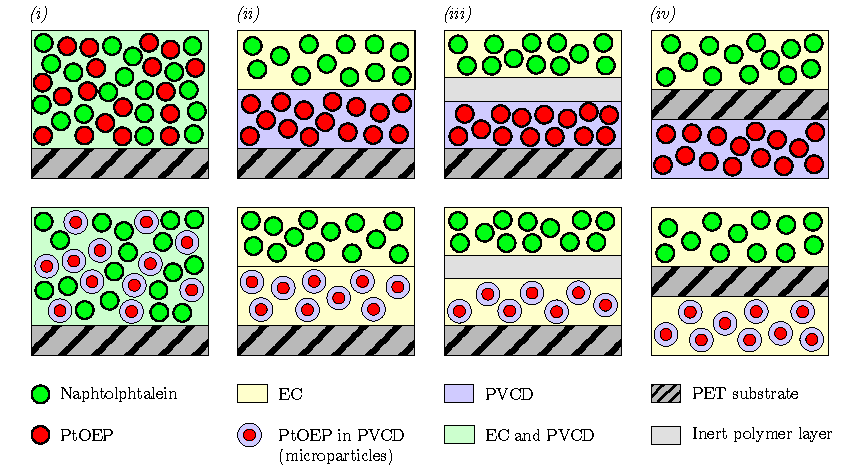
\includegraphics{1_main_matter/thin_film_figures/encasp_pbl/encaps.pdf}
	\caption[Different PtOEP encapsulation strategies.]{Different PtOEP encapsulation strategies for an \gls{ife}-based sensor. $\alpha$-naphtolphtalein is used as pH-sensitive dye while PtOEP acts as reference phosphor. \textbf{Top row:} \textit{(i)}: a solution of $\alpha$-naphtolphtalein in ethyl cellulose (EC) is mixed with a solution of PtOEP in \gls{pvcd} and then cast onto a \gls{pet} substrate, \textit{(ii)}: the two solutions are cast successively on top of each other, \textit{(iii)}: same as \textit{(ii)} but with an intermediate inert polymer layer, \textit{(iv)}: the two solutions are cast on different sides of the \gls{pet} substrate. \textbf{Bottom row:} same as top row, except that the solution of PtOEP in \gls{pvcd} is replaced with a suspension of microparticles of PtOEP encapsulated in \gls{pvcd} into an ethyl cellulose solution. Adapted from Perez \etal{}\cite{perez2009}.}
	\label{fig:thin_film:pbl:encaps}
\end{figure}

Still, despite the latter observation that microparticles seem to perform worse than plain polymer films, significant research efforts have also been deployed to manufacture micro- or nanoparticles for phosphors encapsulation\cite{neurauter2000_phd, kurner2001, bueltzingsloewen2004_phd, edwards2011_phd, ye2012}. This apparent contradiction can be explained by the need for luminescent microparticles in medical imaging\cite{khan2015, feng2023}, or by the need for encapsulated ruthenium complexes for drug delivery\cite{villemin2019}. Additionally, the results of Perez with \gls{pvcd}\cite{perez2009} may not be extrapolated to other luminophore / polymer pairs\cite[Chap.~5]{bueltzingsloewen2004_phd}.

As a side note, we tried to synthesise \gls{rudpp}-doped \gls{pan} nanobeads with Jeanne Beyrle---an intern who worked on the manufacturing of fluorescent thin films for six months during my thesis---following the routes described by Edwards\cite[Chap.~2]{edwards2011_phd} and Ye \etal{}\cite{ye2012}, but without success. In the first case, non-spherical aggregates were obtained that did not encapsulate \gls{rudpp} adequately---the latter redissolved when ethanol was added to the obtained particles. In the second case, polymerisation of acrylonitrile into \gls{pan} could not be achieved, likely due to the presence of inhibitors, although this matter could not be investigated any further due to a lack of time. Ultimately, I stuck with the encapsulation strategy advised by Perez \etal{} in the remainder of this work---\ie{} casting separately the pH-sensitive dye in a hydrophilic permeable polymer and the reference dye in an \gls{o2}-impermeable one.

\section{Selecting the Luminophores}\label{sect:thin_film:select_lumino}

To be usable in an \gls{fdlr} sensing scheme, the two luminophores must meet two main criteria: their excitation spectra must overlap, and $\tau_\mathrm{R}$ should be several orders of magnitude higher than $\tau_\mathrm{A\spminus}$. Additionally, the A$^-$ / AH pH-sensitive fluorophore must have a \pKa{} in the 6--8 range, while R should remain as unaffected by external factors as possible. Ideally, both luminophores must exhibit a good photostability, be reasonably cheap, and possibly available off-the-shelf.

\subsection{Luminophore Review}

A brief literature and internet search was conducted to find luminophores that might meet the above criteria. However, given the vast amount of research available on the topic---a Google Scholar query on \enquote{\texttt{phosphorescence OR fluorescence OR luminescence}} returns over four million entries---and the limited time that was available, the search for luminophore candidates had to be narrowed down to a select few, in a manner that was not strictly objective.

Nevertheless, this research brought into light several luminophore databases, which are summarised in Table \ref{table:thin_film:select_lumino:fluo_db}. These databases may be helpful for anyone eager to continue this work with other luminophores than those selected in the present work. In addition to these databases, one may also refer to the extensive review written by Benezin \etal{}\cite{berezin2010} on the topic of lifetime fluorescence measurements. Going even further, one may also read through several recent publications on the topic of available collections of luminophores, written by the team of Lindsey, Taniguchi, \etal{}\cite{taniguchi2018a, taniguchi2018b}, the very creators and maintainers of the PhotochemCAD database.


% Double hline
\newcommand{\parthline}{\hhline{-------~}}
\newcommand{\doubleparthline}{\hhline{=======~}}
\begin{table}
	\makebox[\textwidth][c]{
		\def\arraystretch{1.25}
		\begin{tabular}{c|c|c|c|c|c|cl}
			Name & \specialcell{Substance\\number} & Spectra & $\Phi_f$ & $\tau_f$  & Sourced & Ref. \\ \doubleparthline
		PhotochemCAD & 339 & Yes & Yes & No & Yes & \cite{taniguchi2018a, taniguchi2018b} & \hspace{0.0em}\rdelim\}{5}{*}[Scholars]\\ \parthline
			Mol. fluo. Appendix & 84 & No$^1$ & Yes & Yes & Yes & \cite{molecular_fluorescence_app} \\ \parthline
			TU Graz & 955 & Yes & Yes$^2$ & Yes$^2$ & Yes$^2$ &\cite{fluodb_tugraz} \\ \parthline
			Max-Planck Institute & 637 & Yes & Yes$^2$ & Yes$^2$ & Yes & \cite{fluodb_maxplanck} \\ \parthline
			McNamara & 1627 & Yes & Yes$^2$ & No & Yes & \cite{fluodb_mcnamara} \\ \doubleparthline
			Thermo Fisher & 470 & Yes & No & No & No &\cite{fluodb_thermofisher} & \hspace{0.0em}\rdelim\}{4}{*}[Industrials]\\ \parthline
			Leica & 257 & No$^1$ & No & No & No & \cite{fluodb_leica} \\ \parthline
			Zeiss & 276 & Yes & No & No & No & \cite{fluodb_zeiss} \\ \parthline
			FluoroFinder & 823 & Yes & No & No & No & \cite{fluodb_fluorofinder}
		\end{tabular}
	}
	\caption[Main luminophore databases and resources available.]{Main luminophore databases and resources available. (1): principal excitation and emission wavelengths provided. (2): not available for all substances.}
	\label{table:thin_film:select_lumino:fluo_db}
\end{table}

\subsubsection{Short-Lived pH-Sensitive Fluorophore}

Many pH-sensitive fluorophores have been developed and deeply studied, both for pH sensors in general\cite{wencel2014}, and for \emph{in vivo} (intra-)cellular imaging in particular\cite{han2010fluo}. Commonly used substances include for instance BCECF, SNARF, BODIPY, and fluorescein derivatives\cite{han2010fluo, boens2012, leguern2020}. However, most of the substances reviewed in the afore-mentioned references are either unavailable off-the-shelf, or extremely expensive---\ie{} often over 1~k\euro/g. Two notable exceptions are pure fluorescein and \gls{hpts}, which are both cheap, pH-sensitive, and easily available off-the-shelf. Their absorption and emission spectra are presented in Figure \ref{fig:thin_film:select_lumino:hpts_fluorescein}. Both fluorophores have quantum yields near unity, but the absorption of fluorescein is almost four times that of \gls{hpts}, hence its markedly higher fluorescence intensity. However, the $pK_A$ of fluorescein is 6.30\cite{lavis2007}, while that of \gls{hpts} is at or above 7.3 depending on the solvent\cite{wolfbeis1983, tranthi2002, sabnis2015} which might make the latter a better candidate for \gls{dlr} applications (see Section~\ref{subsect:conclusion:solid_chemistry}). Consequently, \gls{hpts} was chosen as pH-sensitive fluorophore in my experimentations.

\begin{figure}
	\centering
	\includegraphics{1_main_matter/thin_film_figures/luminophores/tikz/out/fluo_short.pdf}
	\caption[Absorption and emission spectra of the anionic---\ie{} basic---form of \gls{hpts} and fluorescein.]{Absorption and emission spectra of the anionic---\ie{} basic---form of \gls{hpts} and fluorescein. The emission intensity is computed as the peak absorbance times the fluorescence quantum yield. \gls{hpts} was measured in water at a pH of 10 (NaOH solution), fluorescein was measured in ethanol. More information on the pH-dependence of fluorescein may be found in the work of Martin \etal{}\cite{martin1975}, while the case of \gls{hpts} is treated in Section~\ref{subsect:thin_film:select_lumino:hpts}. Data source: PhotoChemCAD database\cite{taniguchi2018b}.}
	\label{fig:thin_film:select_lumino:hpts_fluorescein}
\end{figure}

% leguern2020 pour fluorescein
% boens2012 pour BODIPY

\subsubsection{Long-Lived Reference luminophore}

The choice of the long-lived reference luminophore is much more limited than that of the pH-sensitive short-lived one, because most fluorescence imaging applications use short-lived fluorophores with $\tau_\mathrm{L}$ in the 1--50~ns range\cite{berezin2010, boens2012, houston2018}. Consequently, when the three databases presented in Table \ref{table:thin_film:select_lumino:fluo_db} were searched for luminophores with lifetime exceeding 100~ns, only a few molecules were identified: ref. \cite{molecular_fluorescence_app} yielded pyrene, ref. \cite{fluodb_maxplanck} yielded nothing, and ref. \cite{fluodb_tugraz} yielded eight compounds: four iridium, one palladium, and three platinum complexes, with lifetimes in the 8.5--195~\textmu{}s range. To this list of ten compounds, we added \gls{rudpp}, \gls{rupn} and \gls{rubpy}, three popular long-lived ruthenium complexes. These substances are summarised in Table \ref{table:thin_film:select_lumino:ref_fluo_list}. It should be stressed once again that this selection---although grounded in an in-depth database search---is by no means exhaustive, as exemplified by the many more luminophores compiled by Wang and Wolfbeis in their impressive review of oxygen-sensing materials\cite{wang2014wolfbeis}---some of which have long lifetimes and acceptable quantum yields for our application. Their work might therefore serve as a future source of inspiration, in order to try out other luminophores than the one that I ended up working with.

\begin{table}
	\makebox[\textwidth][c]{
		\small
		\def\arraystretch{1.25}
		\begin{tabular}{c|c|c|c|c|c|cl}
			Name & CAS & \specialcell{$\lambda_{abs} / \lambda_{em}$ \\(nm)} & \specialcell{$\Phi_L \cdot \varepsilon_{H, \lambda_{abs}}$\\(A.U.)} & \specialcell{$\tau_L$ \\ (\textmu{}s)}  & Price & Ref. \\ \doubleparthline
			(C$_S$)$_2$Ir(\textmu{}-Cl)$_2$Ir(C$_S$)$_2$ & N/A & 457 / 587 & 0.21 $\cdot$ 136900 & 13.1 & N/A & \cite{fluodb_tugraz, borisov2007_ultra} & \hspace{0.0em}\rdelim\}{5}{*}[Ir(III)]\\ \parthline
			(C$_N$)$_2$Ir(\textmu{}-Cl)$_2$Ir(C$_N$)$_2$ & N/A & 433 / 567 & 0.30 $\cdot$ 133600 & 9.7 & N/A & \cite{fluodb_tugraz, borisov2007_ultra} \\ \parthline
			Ir(C$_N$)$_2$(acac) & 952584-93-9 & 421 / 545 & 0.53 $\cdot$ 86900 & 8.5 & N/A & \cite{fluodb_tugraz, borisov2007_ultra} \\ \parthline
			Ir(C$_S$)$_2$(acac) & N/A & 472 / 563 & 0.54 $\cdot$ 92800 & 11.3 & N/A & \cite{fluodb_tugraz, borisov2007_ultra} \\ \parthline
			Ir-OEP-CO-Cl & N/A & 404 / 672 & 0.14 $\cdot$ 165000 & 97 & N/A & \cite{fluodb_tugraz} \\ \parthline
			PdTPTBP & 119654-64-7 & 444 / 797 & 0.17 $\cdot$ 264000 & 195 & \href{https://web.archive.org/web/20220204104239/https://www.biomol.com/products/chemicals/biochemicals/meso-tetraphenyl-tetrabenzoporphine-palladium-complex-cdx-t0083-m025}{238~\euro{} / 25~mg} & \cite{fluodb_tugraz, rogers2003} & \hspace{0.1em}\textbf{\}}Pd(II)\\ \parthline
			PtTPTBP & 166174-05-6 & 430 / 770 & 0.7 $\cdot$ 203000 & 53 & \href{https://web.archive.org/web/20220204123237/https://www.frontiersci.com/product/ptii-meso-tetraphenyl-tetrabenzoporphine/}{411~\euro{} / 50~mg} & \cite{borek2007} & \hspace{0.0em}\rdelim\}{3}{*}[Pt(II)]\\ \parthline
			PtOEP & 31248-39-2 & 382 / 647 & 0.41 $\cdot$ 264000 & 90 & \href{https://web.archive.org/web/20220204134104/https://www.frontiersci.com/product/ptii-octaethylporphine-ptoep/}{550~\euro{} / 1~g} & \cite{mills1997_porphyrin, kalinowski2005} \\ \parthline
			PtOEPK & 172617-46-8 & 398 / 760 & 0.12 $\cdot$ 86200 & 61 & \href{https://web.archive.org/web/20220204135427/https://www.porphyrin-systems.de/octaethylporphyrins}{439~\euro{} / 10~mg} & \cite{papkovsky1995, mills1997_porphyrin} \\ \parthline
			\gls{rudpp} & 36309-88-3 & 463 / 618 & 0.37 $\cdot$ 28600 & 6.4 & \href{https://web.archive.org/web/20220204145614/https://www.alfa.com/en/catalog/044123/}{635~\euro{} / 2~g} & \cite{alford1985}$^1$ & \hspace{0.0em}\rdelim\}{3}{*}[Ru(II)]\\ \parthline
			\gls{rupn} & 304695-79-2 & 445 / 595 & 0.02 $\cdot$ 20000 & 0.45 & \href{http://archive.today/2022.02.04-152603/https://www.carbosynth.com/carbosynth/website.nsf/(w-productdisplay)/5C2ABB2E26359101802586A90014C75C}{154~\euro{} / 1~g} & \cite{alford1985} \\ \parthline
			\gls{rubpy} & 14323-06-9 & 286 / 625 & 0.04 $\cdot$ 86100 & 0.64 & \href{https://web.archive.org/web/20220211150558/https://www.ambeed.com/products/50525-27-4.html}{21~\euro{} / 1~g} & \cite{vanhouten1976, muller2012, fluodb_tugraz} \\ \parthline
			Pyrene & 129-00-0 & 241 / 381 & 0.65 $\cdot$ 80000 & 0.45 & \href{https://web.archive.org/web/20220211155425/https://www.chemscene.com/129-00-0.html}{95~\euro{} / 500~g} & \cite{molecular_fluorescence_app, fluodb_maxplanck}
		\end{tabular}
	}
	\caption[A selection of long-lived organo-metallic luminophores.]{A selection of long-lived organo-metallic luminophores. CAS: Chemical Abstracts Service identification number. (1): the given values are sourced from Alford \etal{}\cite{alford1985}. However, it should be noted that a much wider range of values can be found in the literature---see Section \ref{subsect:thin_film:select_lumino:rudpp}. This variability applies to most of the chemicals listed here, so the provided numerical values are indicative only, as they may differ between publications---\eg{} depending on the solvent used, reference standard used for $\Phi_L$ measurement, buffer or additive added, \emph{etc}. Prices are given as of February 2022.}
	\label{table:thin_film:select_lumino:ref_fluo_list}
\end{table}

As one may notice, iridium-based luminophores are not readily available off the shelf, and most palladium and platinum complexes are extremely expensive, with the exception of PtOEP. Thus, we can narrow down our investigations to the following five remaining compounds: PtOEP, \gls{rudpp}, \gls{rupn}, \gls{rubpy} and pyrene. The absorption and emission spectra of these compounds are plotted in Figure \ref{fig:thin_film:select_lumino:long_lived_compilation} along with those of \gls{hpts}.

\begin{figure}
	\centering
	\includegraphics{1_main_matter/thin_film_figures/luminophores/tikz/out/long_lived_compilation.pdf}
	\caption[Absorption and emission spectra of selected luminophores.]{Absorption and emission spectra of selected luminophores. Data source: PhotochemCAD (\gls{hpts} and pyrene), TU Graz (PtOEP, \gls{rupn}, \gls{rubpy}, with quantum yields and extinction coefficients from Table \ref{table:thin_film:select_lumino:ref_fluo_list}), and Bultzingslöwen \etal{}\cite{bultzingslowen2002} (\gls{rudpp}). The area under the absorption and emission spectra of \gls{hpts} \emph{in its anionic form} is coloured in green. Note the difference in vertical scale between the upper and lower part of the figure.}
	\label{fig:thin_film:select_lumino:long_lived_compilation}
\end{figure}

Choosing the optimal long-lived luminophore in these conditions may prove to be a difficult task. Indeed, both the long- and short-lived luminophores must exhibit spectral overlaps---as mentioned in Section~\ref{subsect:choos:dye_based:optical_schemes:dlr_intro}---and the long-lived one must also be reasonably cheap. To address this issue, the following approach was used:
\begin{itemize}
	\item[--] For each of the long-lived fluorophores, a basic sensing scheme was considered. This sensing scheme consists in: an ideal monochromatic light source for excitation, an ideal low-pass reception filter tuned $\delta_\mathrm{LP}=50$~nm above the wavelength of the light source, and located in front of a typical UV-enhanced Si photodiode (\eg{} FDS010, Thorlabs, USA, 5\% of peak sensitivity at 200~nm). The 50~nm difference between the light source and the low-pass filter was set arbitrarily to ensure that---even if the light source is a regular \gls{led} in reality---no light it emits may reach the detector\footnote{This is an ideal case, as actual \glspl{led} may bleed quite significantly even at wavelengths up to 50~nm away from their peak. Here, \enquote{significantly} refers to values as low as $10^{-3}$--$10^{-4}$ times their maximum luminosity, since fluorescence signals are typically quite weak compared to the excitation signals that trigger them. See Section~\ref{ansect:optics:link_budget} for further details on this topic.}.
	\item[--] For a given excitation wavelength $\lambda_\mathrm{ex}$, the emission spectra of the luminophore under study---$\mathcal{S}_\mathrm{L,em}(\lambda_\mathrm{ex})$---is multiplied by its relative absorbance at the excitation wavelength--- $\varepsilon_{\mathrm{L},\lambda_\mathrm{ex}}/\varepsilon_{\mathrm{L},\lambda_\mathrm{abs,max}}$---its quantum yield---$\Phi_\mathrm{L}$---and the so-obtained spectrum is then multiplied by that of the sensitivity of the photodiode---$S_\mathrm{PD}$. Finally, the resulting spectrum is integrated over $\left[ \lambda_\mathrm{ex} + \delta_\mathrm{LP};+\infty \right]$ to yield a unique real value representing the amount of collected light at the photodiode for a given excitation wavelength $\lambda_{ex}$:
	\begin{equation}
		\mathcal{S}_\mathrm{L,PD}(\lambda_{ex}) = \frac{\varepsilon_{\mathrm{L},\lambda_\mathrm{ex}}}{\varepsilon_{\mathrm{L},\lambda_\mathrm{abs,max}}} \cdot \Phi_L \smashoperator{\int_{\lambda = \lambda_\mathrm{ex} + \delta_{LP}}^{+ \infty}} \mathcal{S}_\mathrm{L,em}(\lambda_\mathrm{ex}) \cdot \mathcal{S}_\mathrm{PD}(\lambda_\mathrm{ex})
	\end{equation}
	\item[--] By repeating this procedure for $\lambda_\mathrm{ex}$ values in the 220--500~nm range, we obtain for each luminophore an excitation spectrum $\mathcal{S}_\mathrm{L,PD}$ that takes into account the above-described sensing scheme. The lower bound of this range was limited by the available spectroscopic data, while the upper bound corresponds to the highest bound on \gls{hpts} excitation spectrum (see Section \ref{subsect:thin_film:select_lumino:hpts}). So-obtained excitation spectra are presented in Figure \ref{fig:thin_film:select_lumino:long_lived_bench_nocost}.
\end{itemize}
Of note, these $\mathcal{S}_\mathrm{L,PD}$ spectra are an ideal case wherein \textit{(i)} all the \gls{led}-emitted light would be absorbed by the considered luminophores, \textit{(ii)} no inner filter effect between the luminophores and \gls{hpts} is considered and \textit{(iii)} all the luminophore-emitted light reaches the photodiode. % Still, it allows to take into account both the luminosity of the different luminophores at hand, as well as the fall in photodiode sensitivity towards shorter wavelengths.

\begin{figure}
	\centering
	\includegraphics{1_main_matter/thin_film_figures/luminophores/tikz/out/long_lived_bench_nocost.pdf}
	\caption[Collected light for selected long-lived luminophore and \gls{hpts}.]{Collected light for selected long-lived luminophore and \gls{hpts}. Data source: same as Figure \ref{fig:thin_film:select_lumino:long_lived_compilation}.}
	\label{fig:thin_film:select_lumino:long_lived_bench_nocost}
\end{figure}

At first sight, it seems that PtOEP, \gls{rubpy} and \gls{rudpp} may be good candidates to use as long-lived luminophores in a \gls{dlr} sensing scheme. However, the \emph{cost} of the long-lived luminophores at hand was not taken into account in the above considerations, neither was the availability of affordable light sources in the afore-mentioned 220--500~nm range, nor the fact that---due to the conversion of \gls{hpts} between its acid and basic forms---not all wavelength ranges are suitable for \gls{hpts}-based pH sensing. To overcome these issues, $\mathcal{S}_\mathrm{L,PD}$ was divided by the price per gram of the different luminophores under study. \glspl{led} having short emission wavelengths and a reasonable price were also searched for, and some were found at---or above---275~nm\footnote{For instance the CUD7QF1A \gls{led} (275~nm of peak wavelength, Seoul Viosys, South Korea), which sells below \href{https://web.archive.org/web/20220509144647/https://www.digikey.fr/fr/products/detail/seti-seoul-viosys/CUD7QF1A/9997656}{3\euro} per unit if ordered in large quantities.}, but not below. Finally, the spectral properties of \gls{hpts} require to work either around 380~nm or---better---above 430~nm, \ie{} in spectral ranges wherein the absorption and emission spectra of the protonated and anionic forms of \gls{hpts} differ the most (see Section \ref{subsect:thin_film:select_lumino:hpts}). These different considerations are summarised in Figure \ref{fig:thin_film:select_lumino:long_lived_bench_cost}.

\begin{figure}
	\centering
	\includegraphics{1_main_matter/thin_film_figures/luminophores/tikz/out/long_lived_bench_cost.pdf}
	\caption[Collected light per euro for selected long-lived luminophore and \gls{hpts}.]{Collected light per euro for selected long-lived luminophore and \gls{hpts}. The domain of \gls{led} non-availability is shaded in light grey. The optimal measurement domains with respect to \gls{hpts} spectral properties are shaded in green. The isoemissive point of \gls{hpts} must be avoided at all costs since it makes \gls{hpts}-based pH sensing unfeasible. Data source: same as Figure \ref{fig:thin_film:select_lumino:long_lived_compilation}.}
	\label{fig:thin_film:select_lumino:long_lived_bench_cost}
\end{figure}

Here, pyrene is greatly advantaged by the fact that it is---one, up to three---orders of magnitude cheaper than its competitors. However, it is also the worst compound of the five in terms of luminescence lifetime, having the shortest one, a place that it shares with \gls{rupn}. Additionally, pyrene's luminosity drops significantly in the \gls{hpts}-usable range (green areas in Figure~\ref{fig:thin_film:select_lumino:long_lived_bench_cost}), making it no better than PtOEP, \gls{rudpp}, and \gls{rubpy}, which all outperform it in terms of luminescence lifetime. While \gls{rupn} is clearly out of the race for both intensity \emph{and} lifetime reasons, either PtOEP, \gls{rudpp}, or \gls{rubpy} could be used, since all three of them appear to be good candidates with respect to these latter two criteria. Therefore, a compromise had to be made between luminescence lifetime---for which PtOEP is clearly advantaged before \gls{rudpp} first, and \gls{rubpy} second---and maximum \gls{hpts} fluorescence intensity---for which \gls{rudpp} and \gls{rubpy} are equally advantaged ahead of PtOEP---and \textbf{I finally chose to use \gls{rudpp} in my experiments}, probed above $\sim$430~nm. Now that both the short-lived fluorophore---\gls{hpts}---and long-lived phosphor---\gls{rudpp}---have been selected, they will be briefly presented in the following subsections.

% Ru(bpy)3 % mais tp fluo plus court https://fr.wikipedia.org/wiki/Chlorure_de_tris(bipyridine)ruth%C3%A9nium(II)
% Copper(I) complex % https://www.sigmaaldrich.com/FR/fr/product/aldrich/777692 mais cher aussi
% pyrene spectrum https://omlc.org/spectra/PhotochemCAD/html/079.html

\subsection{HPTS}\label{subsect:thin_film:select_lumino:hpts}

\gls{hpts}---also known as \gls{hopsa}, \gls{hpta}, solvent green 7, or simply pyranine (CAS 6358-69-6, $M=524.39$~g.mol$^{-1}$)---is a green, fluorescent, pH-sensitive dye, which has been used in many a pH or \gls{pco2} sensor\cite{wolfbeis2005, mills2009, dervieux2020dyereview}. Its main properties are summarised in Table \ref{table:thin_film:select_lumino:hpts_prop}, and its molecular structure is given in Equation~\ref{eq:thin_film:select_lumino:hpts_mol}. Contrary to the more simple pyrene from which it is derived---which exhibits a much longer decay time, in the 200~ns range\cite{wolfbeis1983}---its decay time is independent of oxygen quenching\cite{wolfbeis1983, schulman1995} and its fluorescence is pH-sensitive, thanks to its hydroxyl group.

\begin{table}
	\begin{adjustbox}{center}
		\def\arraystretch{1.25}
		\begin{tabular}{c|c|c|c|c}
			\multirow{2}{*}{Property} & \multirow{2}{*}{Notation} & \multicolumn{2}{c|}{Value} & \multirow{2}{*}{References} \\ \cline{3-4}
			& & AH & A$^-$ & \\ \hline \hline
			Acidity constant & \pKa & \multicolumn{2}{c|}{7.3} & \cite{zhujun1984a, schulman1995, bultzingslowen2002, cajlakovic2006} \\ \hline
			Quantum yield & $\Phi$ & \multicolumn{2}{c|}{$\sim$1} & \cite{schulman1995, tranthi2002, kumar2018} \\ \hline
			Decay time & $\tau$ & 4.8$\pm$0.5~ns & 5.3$\pm$0.1~ns & \cite{tranthi2002} \\ \hline
			Absorption peak & $\lambda_\mathrm{abs}$ & $\sim$404~nm & $\sim$460~nm & \cite{zhujun1984a, uttamlal1995, wolfbeis1998, tranthi2002, ge2003, hakonen2008, ge2014} \\ \hline
			\specialcell{Molar extinction\\coefficient at $\lambda_\mathrm{abs}$} & $\varepsilon_{\lambda_\mathrm{abs}}$ & 2.0$\times10^4$~M$^{-1}$.cm$^{-1}$ & 2.4$\times10^4$~M$^{-1}$.cm$^{-1}$ & \cite{sabnis2015} \\ \hline
			Emission peak & $\lambda_\mathrm{em}$ & $\sim$430~nm & $\sim$515~nm & \cite{he1995, tranthi2002, oter2006, chu2008, hakonen2008, chu2009}
		\end{tabular}
	\end{adjustbox}
	\caption[Main properties of \gls{hpts}.]{Main properties of \gls{hpts}. The `$\sim$' symbol is used: \emph{(i)} for the quantum yield, since it has never been reported accurately, and \emph{(ii)} for the wavelengths to allow for a few nanometres of variation from one publication / solvent to another.}
	\label{table:thin_film:select_lumino:hpts_prop}
\end{table}

\begin{equation}\label{eq:thin_film:select_lumino:hpts_mol}
	\schemestart
	\chemname[3ex]{\chemfig{*6(-(*6(-(-NaSO_3)=-(-SO_3Na)=-=))-(*6(--=---))-(*6(=-(-OH)=-(-NaSO_3)=-))--=)}}{Protonated (acidic) form AH}
	\xrightleftharpoons{\pKa = 7.3}
	\chemname[3ex]{\chemfig{*6(-(*6(-(-NaSO_3)=-(-SO_3Na)=-=))-(*6(--=---))-(*6(=-(-{O^-})=-(-NaSO_3)=-))--=)}}{Anionic (basic) form A$^-$}
	\+
	\chemname[3ex]{\ce{H+}}{Proton}
	\schemestop
\end{equation}

\textbf{\pKa, the acidity constant of \gls{hpts},} has often been reported to be about 7.3 at 20$\degree$C. However, the latter value is especially true \emph{in water}. When \gls{hpts} is immobilised in a thin polymer film, \pKa{} appears to shift slightly, ending up lying in the 6.55--8.50 range\cite{schulman1995, hakonen2008}. Similarly, if \gls{hpts} is dissolved in room temperature ionic liquids, its \pKa{} may reach values as high as 9.5--11.2\cite{oter2006}. Further considerations on the effect of ionic strength on the \pKa{} of \gls{hpts} can also be found in Valeur \etal{}\cite[p.~414]{valeur2012molecfluo}.

\textbf{The quantum yield} of \gls{hpts} is often reported to be high, justifying its use, and only a few publications mention it to be near unity, without being overly precise\cite{schulman1995, tranthi2002, kumar2018}.

\textbf{The decay time} of \gls{hpts} has not been measured thoroughly, at least to the best of my knowledge. In the work of Tran-Thi \etal{}\cite{tranthi2002}, values were reported to differ for the protonated (4.8$\pm$0.5~ns) and anionic (5.3$\pm$0.1~ns) forms of \gls{hpts}, although the reported differences lie in the error bars of their measurement. On their part, Wolfbeis \etal{}\cite{wolfbeis1983} reported a constant 5.3~ns decay time, over the full 2--13 pH range. On the contrary, Schulman \etal{}\cite{schulman1995} found decay times of 3.7$\pm$0.1~ns and 5.0$\pm$0.1~ns in immobilised \gls{hpts} equilibrated with 1~M HCl and 1~mM NaOH, respectively. Overall, it is thus unclear whether there is a difference in fluorescence decay time between the protonated and anionic forms of \gls{hpts}. Should such a difference exist in deed, it is nevertheless likely to be quite small---\ie{} below 1--2~ns. % c'est bien les bonnes concentrations pour Schulman

\textbf{The spectral properties of \gls{hpts}} have been reported to a greater or lesser extent by a number of authors---see Table \ref{table:thin_film:select_lumino:hpts_prop}---and the excitation and emission spectra of \gls{hpts} in water can be seen in Figure \ref{fig:thin_film:select_lumino:hpts_spectra}. The protonated form of \gls{hpts} absorbs at $\sim$404~nm and fluoresces at $\sim$430~nm, while its anionic form is excited at $\sim$460~nm and fluoresces at $\sim$515~nm, and an isoemissive point is to be found at $\sim$417~nm\cite{uttamlal1995, oter2008}. However, it has been reported that the polarity of the solvent influences these wavelengths with a red-shift occurring with more polar solvents\cite{barrash1998, tranthi2002}. Furthermore, the use of ionic liquids\cite{oter2006, oter2008}, or the interactions between the dye and its substrate in case of polymer-based, thin film sensors\cite{malins1998, chu2008, chu2009} may also shift the absorption and emission peaks of \gls{hpts}.

\begin{figure}
	\centering
	\includegraphics{1_main_matter/thin_film_figures/luminophores/tikz/out/hpts_spectra.pdf}
	\caption[Absorption and emission spectra of \gls{hpts} in the 1--13 pH range.]{Absorption and emission spectra of \gls{hpts} in the 1--13 pH range. \textbf{Left:} absorption spectra of 22.2~\textmu{}M \gls{hpts} in aqueous 1/15M phosphate buffer. \textbf{Right:} emission spectra of 3.82~\textmu{}M \gls{hpts} when excited at 454~nm. Data source: Wolfbeis \etal{}\cite{wolfbeis1983}.}
	\label{fig:thin_film:select_lumino:hpts_spectra}
\end{figure}

\textbf{Ageing and photobleaching of \gls{hpts}} have seldom been reported in the literature for \gls{co2} sensing\cite{borisov2007}. Recent work by Nairn \etal{}\cite{nairn2015} aiming at characterising \gls{hpts} photobleaching revealed that---although \gls{hpts} is considered a fairly stable compound by a number of authors\cite{wolfbeis1998, bultzingslowen2002, cajlakovic2006}---it is nonetheless subject to photobleaching to some extent. Nairn \etal{} indeed reported degradation time constants of only a few hours upon continuous exposure to sunlight.

\textbf{Solubility of \gls{hpts}} has been reported in a wide range of solvents, although quantitative data are sparsely available. For instance, Bobe \etal{} reported \gls{hpts} solubility constants of at least 3~{\textmu}M in \gls{dmf}, \gls{dmso}, ethanol, and methanol\cite{bobe2014} ($\sim$1.6~mg.L$^{-1}$). Other sources report up to 300~g.L$^{-1}$ in water, and 100~g.L$^{-1}$ in methanol\cite{chembookpyranine}. An extensive list of solvents---among which \gls{ipa}, acetone, acetonitrile, ethylene glycol, and \gls{thf}---can also be found in the work of Barrash \etal{}\cite{barrash1998}, although no precise solubility figures are given.

\subsection{The Ruthenium(II) Complex}\label{subsect:thin_film:select_lumino:rudpp}
\glsreset{rudpp}

The Ruthenium(II) complex that will be used as a reference luminophore is \gls{rudpp} (CAS 36309-88-3, $M=1169.17$~g.mol$^{-1}$). \gls{rudpp} is an organometallic phosphorescent dye with a long lifetime, and whose luminescence is strongly quenched by \gls{o2}. Its main properties are summarised in Table \ref{table:thin_film:select_lumino:rudpp_prop} and its molecular structure as well as excitation and emission spectra are given in Figure \ref{fig:thin_film:select_lumino:rudpp_mol_spectra}.

\begin{table}
	\centering
	\def\arraystretch{1.25}
	\begin{tabular}{c|c|c|c}
		{Property} & {Notation} & {Value} & {References} \\ \hline \hline
		Quantum yield & $\Phi$ & 0.2--0.75 & \cite{alford1985, xu1994} \\ \hline
		Decay time & $\tau$ & 0.8--6.40~\textmu{}s & \cite{alford1985, bacon1987, xu1994, liebsch1999, baker2000} \\ \hline
		Absorption peak & $\lambda_\mathrm{abs}$ & $\sim$430--467~nm & \cite{alford1985, bacon1987, baker2000, mills2013} \\ \hline
		\specialcell{Molar extinction\\coefficient at $\lambda_\mathrm{abs}$} & $\varepsilon_{\lambda_\mathrm{abs}}$ & 2.86$\times10^4$~M$^{-1}$.cm$^{-1}$ & \cite{alford1985} \\ \hline
		Emission peak & $\lambda_\mathrm{em}$ & $\sim$604--618~nm & \cite{alford1985, bacon1987, baker2000, mills2013} 
	\end{tabular}
	% compound 40 in alford 1985
	\caption{Main properties of \gls{rudpp}.}
	\label{table:thin_film:select_lumino:rudpp_prop}
\end{table}

\begin{figure}[h]
	\centering
	\def\mrusep{2mm}
	\def\mrumult{2}
	\adjustbox{width=60mm, valign=c}{
		\chemfig{
			Ru^{2+}
			(<:#(\mrusep,\mrusep)[::30,\mrumult]N*6(-(*6(-(*6(-N=-=(-*6(-=-=-=))--))=-=--))=-(-*6(-=-=-=))=-=-))
			(-#(\mrusep,\mrusep)[::90,\mrumult]\hphantom{N})
			(<:#(\mrusep,\mrusep)[::150,\mrumult]N*6(-(*6(-(*6(-N=-=(-*6(-=-=-=))--))=-=--))=-(-*6(-=-=-=))=-=-))
			(<#(\mrusep,\mrusep)[::210,\mrumult]\hphantom{N})
			(-#(\mrusep,\mrusep)[::270,\mrumult]N*6(-(*6(-(*6(-N=-=(-*6(-=-=-=))--))=-=--))=-(-*6(-=-=-=))=-=-))
			(<#(\mrusep,\mrusep)[::330,\mrumult]\hphantom{N})
			(-[::305,7,,,,transparent]2\cdot Cl^{-})
	}}
	\hspace{2mm}
	\includegraphics[valign=c]{1_main_matter/thin_film_figures/luminophores/tikz/out/rudpp_spectra.pdf}
	\caption[\gls{rudpp} molecular structure and excitation and emission spectra.]{\textbf{Left:} \gls{rudpp} molecular structure. \textbf{Right:} excitation and emission spectra of \gls{rudpp} immobilised in polymer nano-beads. Redrawn from Bultzingslöwen \etal{}\cite{bultzingslowen2002}.}
	\label{fig:thin_film:select_lumino:rudpp_mol_spectra}
\end{figure}

\textbf{The \gls{o2} fluorescence quenching of \gls{rudpp}} has been a long known phenomenon, which has been exploited to elaborate \gls{o2} probes and sensors since the nineteen eighties\cite{bacon1987, baker2000, xu1994, mills2013}. However, this quenching becomes an unwanted cross-sensitivity when developing a \gls{co2} sensor. Consequently, several authors proposed dye encapsulation techniques---notably into \gls{pan} films or micro-beads\cite{liebsch1999, bultzingslowen2002, burke2006, cajlakovic2006}---to avoid the influence of \gls{o2} on \gls{rudpp} fluorescence. Of note, some of the latter references---\eg{} Liebsch \etal{}\cite{liebsch1999}---did not study \gls{rudpp} di\emph{chloride} strictly speaking, but \gls{rudpp} di\emph{hexafluorophosphate} or other anionic variants instead.

\textbf{The quantum yield} of \gls{rudpp} has seldom been reported and depends both on the solvent in- and on the temperature at which it is measured. Values reported in ethanol\cite{alford1985} or butyronitrile\cite{kapturkiewicz1995} are rather low---0.2 and 0.366, respectively---while entrapment in polymers can raise it to as much as 0.75\cite{alford1985}. Xu \etal{}\cite{xu1994} reported a more laconic value of 0.5, although their primary source---Nakamaru \etal{}\cite{nakamaru1979}---could not be retrieved, seemingly lost in the sands of time. Again, \gls{o2} quenching plays its role in the quenching of the emission intensity of \gls{rudpp}\cite{mills2013}.

\textbf{The decay time} of \gls{rudpp}---as its quantum yield---also strongly depends on the solvent with values near 5.34~\textmu{}s in deoxygenated methanol\cite{demas1977}, 6.9~\textmu{}s in \gls{pvc}\cite{alford1985} but closer to 0.8~\textmu{}s in aqueous solution\cite{liebsch1999}. This lifetime was also reported to decrease notably with temperature\cite{bacon1987, liebsch1999}, and---of course---with oxygen quenching\cite{bacon1987}.

\textbf{The luminescence properties of \gls{rudpp}} consist in a broad excitation spectrum in the blue end of the visible spectrum ($\sim$400--500~nm) and a narrower emission peak in the yellow-red ($\sim$550--650~nm). The emission spectrum of \gls{rudpp} has been reported to blue-shift once entrapped into a polymer film\cite{alford1985} and to red-shift with an increase in temperature\cite{baker2000}\footnote{Here \enquote{blue-shift} and \enquote{red-shift} were used instead of the more literary \emph{hypsochromic} and \emph{bathochromic} shift denomination, so as to remain comprehensible to a novice reader.}.

\textbf{Solubility of \gls{rudpp}} has been reported in a 4:1 ethanol / methanol mixture\cite{alford1985} and in methanol\cite{demas1977} without specific numerical values, and up to 400~{\textmu}M ($\sim$0.47~g.L$^{-1}$) in ethanol\cite{baker2000}, 40~g.L$^{-1}$ in chloroform\cite{khan2015} or approximately 33~mg.L$^{-1}$ in dichloromethane\cite{xu1994}. In the course of my experimentations, I observed a fast---\ie{} below one minute---dissolution at 9.0~mM ($\sim$10.5~g.L$^{-1}$) in both \gls{dmf} and \gls{dmso}, and a slower one---\ie{} several hours---in a 3:1 ethanol / water mixture at 4.5~mM ($\sim$5.2~g.L$^{-1}$). These indicative durations and solubility values were observed during the preparation of 5--10~mL of solutions stirred at 60{\degree}C---see Section~\ref{subsect:thin_film:experimental:materials} for chemicals origin.

\section{Selecting the Polymers}\label{sect:thin_film:select_poly}

The use of two luminophores with very distinct purposes calls for two corresponding polymers with very distinct properties: one of them must act as an oxygen barrier in order to encapsulate the oxygen-sensitive \gls{rudpp}, hence it should have a very low gaseous solubility and diffusivity. On the contrary, the other one must be highly hydrophilic / hygroscopic, and facilitate the diffusion of \gls{co2}, in order to allow for a good acid-basic conversion of \gls{hpts} and a fast detection of the latter gas. Additionally, those two polymers must be optically clear, reasonably cheap, and solvent-compatible with the involved luminophores as well as with one another---\ie{} the solvent used to dissolve one polymer must not dissolve the other, and \textit{vice versa}.

Note that considerations relative to the thermal, oxidative, (photo)chemical, or physical degradation of the said polymers---while relevant in the general case of polymer benchmarking---were set aside in the following developments since the obtained thin films will operate at room-temperature and without excessive mechanical load. Furthermore, the involved luminophores are orders of magnitude more sensitive to (photo)chemical and oxidative degradations than the polymers that will embed them---see Sections~\ref{subsect:thin_film:encaps:photobleaching} and \ref{subsect:thin_film:experimental:pbl}. Consequently, the luminophores in the polymer films will have completely photobleached long before the polymers which encapsulate them begin to suffer from the ravages of time and radiation. Still, the curious reader may refer to Korotcenkov for further discussions on polymer (long-term) stability\cite[Chap.~9]{korotcenkov2014}.

\subsection{\texorpdfstring{\gls{rudpp}}{Rudpp} Encapsulating Polymer}\label{subsect:thin_film:rudpp_poly}

\subsubsection{Polymer Selection}

In choosing the \gls{rudpp} encapsulating polymer, I focused on having the lowest permeability as possible towards oxygen. A compilation of various bibliographic resources on the topic of polymer permeability towards oxygen can be found in Table \ref{table:thin_film:select_poly:polymer_o2_perm}.

\begin{table}
	\small\centering\def\arraystretch{1.25}
	\makebox[\textwidth][c]{
		\begin{tabular}{c|c|c|c}
			\specialcell{Nb. of polymers\\reviewed} & \specialcell{Lowest $P$\\(barrer$^{(a)}$)} & {Corresponding Polymer} & {Ref.} \\ \hline \hline
			6 & 2.34 & polyethylene (low density) & Yasuda \etal{}\cite{yasuda1966} \\ \hline
			10 & 0.43 & poly(butylene adipate) polyester-based polyurethane & Wang \etal{}\cite{wang2012} \\ \hline
			5 & 0.16 & \gls{pmma} & Yang \etal{}\cite{yang1981} \\ \hline
			22 & 3.28$\times10^{-2}$ & polyvinyl fluoride (PVF) & Aiba \etal{}\cite{aiba1968} \\ \hline
			19 & 4.0$\times10^{-3}$ & \gls{pvcd} & Surgi \etal{}\cite{surgi1989} \\ \hline
			84 & 2.8$\times10^{-3}$ & BTDA-p,p'-DAS & Koros \etal{}\cite{koros1992} \\ \hline
			11 & 5.61$\times10^{-4}$ & \gls{ppta} & Kanehashi \etal{}\cite{kanehashi2010} \\ \hline
			57 & 2.0$\times10^{-4}$ & \glsreset{pan}\gls{pan} & Sangaj \etal{}\cite{sangaj2004} \\ \hline
			$\sim$400 & 3.7$\times10^{-5\;(b)}$ & \gls{evoh} & McKeen \cite[p. 187]{mckeen2017}
		\end{tabular}
	}
	\caption[Bibliographic review of the permeability of polymers towards oxygen.]{Bibliographic review of the permeability $P$ of polymers towards oxygen. (a): 1~barrer is equal to 10$^{-10}\times$cm$^3_{\text{STP}}\cdot$cm$\cdot$cm$^{-2}\cdot$s$^{-1}\cdot$cmHg$^{-1}$. (b) an even lower value of 3.1$\times10^{-6}$ have been reported by Massey\cite[p. 267]{massey2003} for 140{\degree}C heat-treated \gls{evoh}.}
	\label{table:thin_film:select_poly:polymer_o2_perm}
\end{table}

Of note, this table should be taken with a pinch of salt, because several authors reported widely varying values for the same substance---\eg{} depending of the considered nuance\footnote{The word \emph{nuance} is loosely used here to denote constitutive variations in commercial grades of polymers. These variations can correspond to different amounts of additives, degrees of polymerisation, of proportions of the different monomers involved (in case of a copolymer). The curious reader may refer to McKeen for further information on this topic\cite[Chap.~2]{mckeen2017}.}, EVOH permeability can be multiplied more than tenfold\cite[p.~185]{mckeen2017}. As such, it is not rare to see reports of permeability values spanning more than one order of magnitude for a given polymer, even at a single given temperature\cite[App. II]{massey2003}. It should also be noted that both temperature and humidity greatly influence polymers' permeability---\eg{} \gls{evoh} oxygen permeability can be multiplied by up to 63 from 0\% \gls{rh} to 100\% \cite[pp. 264--5]{massey2003}, similar orders of magnitude are also observed when increasing the temperature from room temperature (20--25{\degree}C) to the 25--50{\degree}C range\cite[App. II]{massey2003}. Most of the time, the values reported in \ref{table:thin_film:select_poly:polymer_o2_perm} are given in dry air and at room temperature, although this is not always the case due to the multiplicity of sources. The reader is therefore highly encouraged to delve into the afore-mentioned references for precise comparisons. From this crude bibliographic research, \gls{ppta}, \gls{pan} and \gls{evoh} were considered for further investigations due to their outstandingly low permeability values.

At first, \gls{ppta}---better known to the general audience under DuPont's commercial name \emph{Kevlar}---was discarded for two main reasons:
\begin{enumerate}
	\item It is insoluble in almost all solvents but sulphuric acid\cite{sokolova1974, arpin1977}\footnote{For the sake of completeness, some organic solvents---such as dimethylacetamide or (m)ethylformamide---may also work in conjunction with a variety of salts\cite{westerhof2009phd}.}, hence it is a polymer especially difficult to work with, requiring multiple steps to turn it into a film\cite{flood1982, fujita1989}.
	\item \Gls{ppta} films, if transparent when thin enough, are not optically clear---having been reported as gold or yellow in colour\cite{fujita1989, weinkauf1992, lu2018}. This yellowish colouring---which is similar to that of the well-known Kevlar fabric---prevents their use in the envisioned fluorescence setup, since it indicates a strong light absorption in the blue wavelengths. Although absorption spectra of micrometer-thick \gls{ppta} thin films could not be found in the literature, the work of Yang \etal{} indeed indicates significant light absorption for \gls{dmso} / Kevlar nanofibres dispersion in the 300--500~nm wavelength range\cite{yang2015}. Furthermore, Kevlar also fluoresces when excited in the 300-500~nm range, re-emitting light in the 450--700~nm region\cite{penn1979}.
\end{enumerate}

Then, \gls{pan} was preferred over \gls{evoh} for its better tolerance towards humidity. Indeed, while \gls{pan} permeability only increases by 10--20\% at high humidity levels\cite{allen1977}, that of \gls{evoh} increases dramatically, as stated above. Ultimately, this results in \gls{evoh} having a far higher permeability than \gls{pan} in water-saturated air\cite{park1985}, a condition that is met at occluded human skin---see Section~\ref{sect:tcco2:skin_mes:rh}.

\subsubsection{\texorpdfstring{\gls{pan}}{PAN}}

\gls{pan} comes in the form of a white powder, which is highly soluble in a variety of solvents, notably \gls{dmf}, \gls{dmso}, nitric and sulphurous acid, as well as aqueous solutions of sodium thiocyanate (NaSCN) and zinc chloride (ZnCl$_2$). Various reports indicate solubilities of at least 5--6m\%\footnote{The `m\%' notation is used for mass percentage, \aka{} mass fraction or percentage by weight, and sometimes also noted `wt.\%' or `\%w/w'---although this can be seen as a misuse of the term weight\cite{se_mass_vs_weight}.} for all the afore-mentioned solvents\cite{kawai1964, hattori1996}, and much higher figures have even been reported for \gls{dmf}, with solubilities in the 20--25m\% range\cite{iovleva2001, tan2008}. Further still, it has been suggested that there was no upper limit to the solubility of \gls{pan} in \gls{dmf}, apart from the difficulty of thoroughly homogenising the polymer / solvent mixture---especially for \gls{pan} concentrations above 25m\%\cite{ham1954, tan2008}. Indeed, \gls{pan} powder tends to swell when exposed to \gls{dmf}, forming a gel layer which prevents the solvent from reaching the remaining undissolved powder\cite{eom2020}, a behaviour that I also observed in the lab (\gls{pan} powder, 99.5\% acrylonitrile, $M \approx 230$~kg.mol$^{-1}$, AN316010, Goodfellow, UK). Thus, \gls{pan} concentrations above 20m\% are difficult to come by in practice, and hardly workable because of their extreme viscosity. Interestingly, Eom \etal{} reported that this swollen gel layer phenomenon is far less marked when using \gls{dmso} instead of \gls{dmf}\cite{eom2020}. Therefore, even if---for historical reasons---all my experimentations were conducted with \gls{dmf} as a solvent for the \gls{rudpp} / \gls{pan} mixture, \gls{dmso} could have probably also been envisioned\footnote{In practice, this may not be that simple: several tests were performed in this direction and, while dissolving \gls{rudpp} (9.0~mM) and \gls{pan} (10m\%) in \gls{dmso} proved relatively straightforward (<8~h at 70{\degree}C), the resulting films curled in on themselves while drying, delaminated from the glass substrate they were cast onto, and developped a whitish opaque tint. A quick assessment of photobleaching led to results similar to those obtained with \gls{dmf}. Finally, it should be noted that \gls{pet} is soluble in \gls{dmso}\cite[p~13-9]{crchandbook95th2014}, which further refrained me from using the latter in the end, since \gls{pet} was a candidate substrate for the final thin films instead of glass---see Section~\ref{sect:conclusion:substrate}.}.

% Pas certain, j'avais lu qq part que la coagulation se passait "mieux" (je sais plus de quel point de vue) avec du DMF qu'avec du DMSO.

The curious reader may have a look to references \cite[pp. 393--443]{cook1984} and \cite[Chap. 4]{olabisi2016} for further considerations about \eg{} \gls{pan} history, polymerisation process, mechanical properties, thermal stability, or morphology, to name a few.

% Hattori 1996 : 5% in DMF, DMSO, NaSCN, dimethylacetamide
% Kawai 1963 : 6g/dl in ZnCl2 / H2O, nitric and sulphuric acid
% 20% in DMF (Tan 2008)
% no limit even if tedious above 25% Ham 1954
% PAN solubility
% up to 25% in DMF iovleva2001
% kamide2002 note que le degré de tacticité du PAN joue sur sa solubilité (quoi que ça veuille dire)
% Dans textile fiber : le PAN garde ses propriétés mécaniques en cas d'humidification !
% Dans Handbook of thermoplastics : cheat sheet p148

\subsection{Breathable Polymer}\label{subsect:thin_film:breath_poly}

\subsubsection{Polymer Selection}\label{subsect:thin_film:breath_poly:poly_select}

\textit{A priori}, the choice of the polymer used to embed the pH-sensitive dye should be guided by the fact that this polymer has both a good \gls{co2} permeability---so that \gls{co2} can easily dissolve from the skin into the polymer matrix---and hygroscopy---so that water molecules entrapped in its bulk may contribute to the hydration of collected \gls{co2} molecules. This breathable polymer should in addition have decent optical transparency and mechanical properties, for optical probing and cutaneous application, respectively. Yet, despite the fact that Aguayo-L\'opez \etal{} mention that choosing a more hydrophilic polymer for the preparation of dye-based thin film sensors should yield a better stability, their results show satisfying performance using either ethyl cellulose or \gls{hpmc} with no major difference between the two, in spite of the fact that the latter is more hydrophilic than the former\cite{aguayolopez2014}. Additionally, McMurray put forth as far back as 1992 that the water molecules available for \gls{co2} hydration may predominantly originate from the quaternary ammonium cation used as phase transfer agent, rather than from the encapsulating polymer matrix\cite{mcmurray1992}, a hypothesis grounded in the work of Landini \etal{}, although the authors indicate that it may be the complementary anion and not the quaternary ammonium anion by itself that interacts with water molecules\cite{landini1978}.

That being said, since McMurray's hypothesis has---to the best of my knowledge---neither been confirmed nor infirmed to date, I considered that the hygroscopy of the encapsulating polymer \emph{may} influence the behaviour of thin film \gls{co2} sensors. In order to better understand the phenomena of hydrophily and hygroscopy of polymers, a quick bibliographic search about those phenomena was performed. However, this research is mainly presented here for reference, as well as to hopefully provide the reader with a few insights on this broad topic. Indeed, I ended up making my choice between the narrow range of polymers which had been already successfully tried out by other authors for \gls{co2} sensing to stay on the safe side---see Section~\ref{subsect:thin_film:breath_lite}---though \mfrin{}further research on this topic is definitely needed---notably to investigate the validity of McMurray's hypothesis.

\paragraph{Of Polymers and Water}\mbox{}\\

Polymers, in addition to the concepts of water solubility---\ie{} the ability to dissolve into water, characterised by the solubility coefficient or solubility parameter\cite{gong2007}---or water (vapour) permeability---\ie{} the ability to let water molecules diffuse through it, characterised by various physical quantities such as water vapour transmission rate, permeability, solubility and diffusivity\cite{chapter4_solubility}---can also be defined by their hydrophilic or hygroscopic nature. These two notions, however, may have different meanings depending on the authors and research fields. Indeed, \emph{hydrophilicity} can be used to describe distinct properties: as a synonym for hygroscopy or solubility, but also to describe the surface-wetting properties of water onto a given material---often characterised by the contact angle of water droplets at its surface\cite{drelich2011, corsaro2021}. On its part, the meaning of \emph{hygroscopy} is relatively consensual, and relates to the ability of a polymer to embed water molecules into its bulk. It is often characterised by the influence of \gls{rh} on mass change---often simply denoted as \enquote{water uptake} or \enquote{moisture content}, and expressed as a percentage of the dry polymer mass\cite{valenzuela2011, vidovic2013}---swelling\cite{grossutti2020}, or glass transition temperature shift\cite{patel2022_part1, patel2022_part2, patel2023_part3}.

Those phenomena have been extensively studied, either theoretically by means of diffusion models\cite{vanderwel1999, chapter4_solubility} and---more recently---molecular simulations\cite{kulasinski2015, kulasinski2016}, or practically \textit{via} myriads of specific studies on the water uptake, swelling, or wettability of polymers---a simple Google Scholar request on \enquote{\texttt{polymer AND ("water uptake" OR (water AND swelling) OR hygro\-scopy OR hydrophilic) AND review}} yields over one million results. This vast literature corpus originates from the ubiquitous presence of water on earth coupled to the ever-growing polymer use in industrial applications\cite[Fig. S1]{geyer2017}, and recent research interests on water-polymer interactions include for instance food packaging\cite{asim2022}, edible coating\cite{mishra2010}, microencapsulation for ink printing or drug delivery\cite{rogers2012}, water-soluble capsules for clinical use\cite{yang2020capsule}, anti-fouling coatings\cite{rana2010}, or water harvesting in dry environments\cite{guo2022}, to name a few.

Yet, this diversity of applications and research perspectives makes it exceedingly difficult for the novice to provide a comprehensive and usable picture of water-polymer interactions. Even specialised textbooks dedicated to polymer permeability such as Massey's 2003 \textit{Permeability Properties of Plastics and Elastomers}\cite{massey2003} or McKeen's update of the latter\cite{mckeen2017} largely ignore cellulose derivatives, for instance\footnote{Massey only mentions the oxygen permeability of methyl cellulose and \gls{hpmc} without much detail on the materials (molar mass, methoxy content, \etc{}), while McKeen focuses solely on raw, nitro, and ethyl cellulose, as well as cellulose acetate, but without mentioning \gls{hpmc}.}. Worse still, any attempt to paint such a picture seems doomed to failure, for there is no such thing as \enquote{a polymer}, from a water-interaction perspective. Indeed, while there are of course major differences in hygroscopy based on a polymer's monomer unit---\eg{} between ethyl cellulose, hydroxypropyl cellulose, or \gls{hpmc}\cite{patel2022_part2}---there are also considerable variations depending on the polymer's degree of polymerisation\cite{patel2022_part1, thijs2007} or crystallinity\cite{hatakeyama1998}, temperature\cite{patel2022_part1, patel2022_part2, patel2023_part3}, or presence of additives\cite{mishra2010, khwaldia2013, mahadevaiah2017}---\eg{} plasticisers\footnote{As well as the degree of polymerisation of the considered polymer\cite{aydinli2000}.}---not to mention the measurement variability from one publication to the other, which can be induced by inappropriate protocols\cite{valenzuela2011}. Facing this growing number of parameters and the factorial explosion of possible combinations that ensues, taking into account my relative ignorance on this complex topic, and because of the limited time I had to complete this doctoral work, I chose to stay on the safe side, and to select a polymer / plasticiser combination among those used in the literature for thin film \gls{co2} sensing specifically.

\paragraph{In the \texorpdfstring{\gls{co2}}{CO2}-Sensing Literature}\label{subsect:thin_film:breath_lite}\mbox{}\\

Table~\ref{table:thin_film:select_poly:breathable_polymer} presents a literature review of breathable polymers used for dry dye-based thin film \gls{co2} sensing. Because of its moderate sensitivity towards humidity, plurality of reporting works, and affordability, \gls{hpmc} was finally chosen to act as a breathable polymer for \gls{hpts} encapsulation, plasticised by Tween 20. Again, it must be emphasised that this choice has its share of arbitrariness, and other solutions could prove to be better alternatives. In particular, cellulose acetate and cellulose acetate butyrate, or \gls{pva} may be interesting alternatives to \gls{hpmc} given their high \gls{co2} permeability and water vapour transmission rate\cite{tock1983}.

\begin{table}
	\small\centering\def\arraystretch{1.25}
	\makebox[\textwidth][c]{
		\begin{tabular}{c|c|c|c}
Polymer & Plasticiser & \specialcell{Humidity influence\\on \gls{co2} readings} & {Ref.} \\ \hline \hline
Cellulose fibres & None & Yes, strong & \cite{wang2020} \\ \hline
EG / PEG & TBP & Yes, moderate & \cite{cajlakovic2006} \\ \hline
Ethyl cellulose & \specialcell{DOP\\TBP\\TOP\\Tween 20} & Yes, strong & \specialcell{\cite{aguayolopez2014, amao2004, amao2005a, bultzingslowen2003, chu2017}\\\cite{ fernandezramos2019, fritzsche2017, hakonen2008, mills1997, nakamura2003}\\\cite{neurauter1999, oter2008, perez2009, pfeifer2020}\\\cite{staudinger2018, wolfbeis1988, wolfbeis1998}} \\ \hline
Hydroxyethyl cellulose & Glycerol & Yes, moderate & \cite{cajlakovic2006} \\ \hline
\gls{hpmc} & Tween 20 & Yes, moderate & \cite{aguayolopez2014, fernandezramos2018, fernandezramos2019} \\ \hline
Ormosil & None & Yes, strong & \cite{bultzingslowen2002, chu2008, chu2009, dansby2010, malins1998, segawa2003} \\ \hline
PolyIBM & TBP & N/A & \cite{amao2005b} \\ \hline
PMMA / MOF & DOP & N/A & \cite{zeyrek2021} \\ \hline
metal-loaded PVA & None & None for \gls{rh} > 25--50\% & \cite{fernandezsanchez2007} \\ \hline
PVCD & TBP & Yes (stability?) & \cite{perez2009} \\ \hline
Silicone & None & Conflicting sources$^\text{(a)}$ & \cite{ge2003, burke2006, borisov2007}
		\end{tabular}
	}
	\caption[Bibliographic review of breathable polymers.]{Bibliographic review of breathable polymers that were used for \gls{co2} sensing. EG: Eudragit. PEG: polyethylene glycol. TBP: tributylphosphate. DOP: dioctylphtalate (\aka{} bis(2-ethylhexyl) phthalate). TOP: tris(ethyl-hexyl) phosphate. PolyIBM: poly(isobutyl methacrylate). PMMA: poly(methyl methacrylate). MOF: metal organic framework. PVA: polyvinyl alcohol. PVCD: polyvinylidene chloride. Silicone: \gls{pdms} and derivatives thereof. (a): two authors reported a marked influence of water while Borisov \etal{} report that one of their sensors \enquote{still responds to carbon dioxide at relative humidities close to 0 and shows sensitivity similar to that in humidified gas.}\cite{borisov2007}.}
	\label{table:thin_film:select_poly:breathable_polymer}
\end{table}

\subsubsection{\texorpdfstring{\gls{hpmc}}{HPMC}}\label{subsect:thin_film:poly_hpmc}

\gls{hpmc}---\aka{} hypromellose, or under the trade name \textit{Methocel}---has a cellulosic backbone from which several hydroxyl groups have been substituted by either methoxy or hydroxypropyl groups\cite[Fig.~1]{li2005}. As such, it is often characterised by both its degree of polymerisation---or molar mass---and by the percentage of its hydroxyl groups that have been substituted by methoxy or hydroxypropyl groups\cite[Table~I]{archer1991}. \gls{hpmc} comes in the form of a white powder that is extensively soluble in water---\ie{} up to at least 60m\%\cite{pekel2004}---but also in water-ethanol mixtures\cite{fernandezramos2019}, \gls{dmso}, benzyl alcohol and formamide\cite{archer1991}. However, just as with \gls{pan} dissolution in \gls{dmf}, \gls{hpmc} also tends to form a gel when dissolving into water\cite{li2005}, making it particularly difficult to reach concentrations above a few tens of percent. Additionally, \gls{hpmc} is reputed to be poorly soluble in hot water, exhibiting thermoreversible gelation---\ie{} forming a gel at high temperature which dissolves upon cooling---a phenomenon which depends on both the \gls{hpmc} concentration and degree of hydroxypropyl substitution\cite{ford1999}. Cloud points are usually reported to lie in the 37--70{\degree}C range, depending on the type---\ie{} percentage of methoxy and hydroxypropyl groups---and concentration of \gls{hpmc} used. In the lab, no cloud point nor gelation were observed with a 20m\% concentration at 55{\degree}C in a 1:1 water / ethanol mixture or with a 10m\% concentration at 60{\degree}C in a 2:1 water / ethanol mixture (\gls{hpmc} powder, 29m\% methoxy, $M \approx 10$~kg.mol$^{-1}$, 423238, Sigma-Aldrich, USA). Dissolution was always quick---less than 2~h---but 20m\% solutions were exceedingly thick\footnote{No viscometer was available in the lab, but 20m\% \gls{hpmc} solution in 1:1 water / ethanol mixture were estimated to be in the 10,000-50,000~cP range using visual scales---\ie{} akin to molten chocolate just before solidifying, very thick honey, or ketchup, for instance---flowing with great difficulty and immobilising the magnetic stirrer.}, making them difficult to work with.

\section{Optoelectronics}\label{sect:thin_film:opto_elec}

A synoptic view of the opto-electronic system that was used to probe the manufactured \gls{co2}-sensing thin films can be seen in Figure~\ref{fig:thin_film:opto_elec:synoptic}. The following sections detail separately the optical and electronic aspects of this setup.

\begin{figure}
	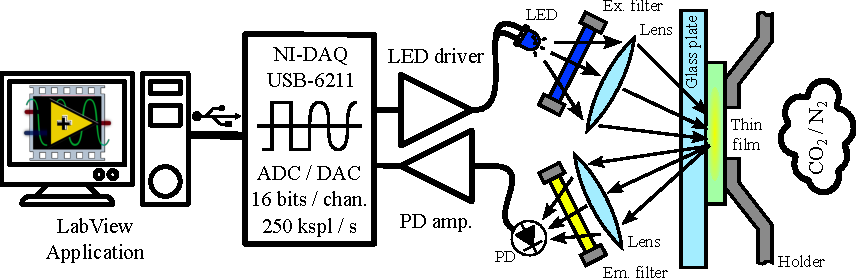
\includegraphics{1_main_matter/thin_film_figures/optoelectronics/synoptic}
	\caption[Synoptic view of the acquisition system.]{Synoptic view of the acquisition system. The computer runs a LabView application which communicates with the acquisition board. The latter in turn sends an excitation signal to the \gls{led} through the \gls{led} driver. The emitted light is focused through a shortpass excitation filter onto the fluorescent thin film that is placed inside a gas-tight box, into which the \gls{co2} concentration, temperature and humidity levels can be regulated. The re-emitted light is then collected and passed through a longpass emission filter to reach the photodiode (PD). The photodiode's signal is then amplified and read back by the acquisition board.}
	\label{fig:thin_film:opto_elec:synoptic}
\end{figure}

\subsection{Optical Setup}

\subsubsection{Spectral Configuration}

The 450~nm blue \gls{led} (LED450L, Thorlabs, USA) is focused through a 450~nm cut-off, shortpass, OD5, excitation filter (FES0450, Thorlabs) onto the \gls{co2}-sensitive fluorescent thin film. The re-emitted light is passed through a 500~nm cut-off, longpass, OD5, emission filter (FEL0500, Thorlabs), and collected onto a silicon photodiode (SM05PD1A, Thorlabs). The fluorescence excitation and emission filters, \gls{led}, and photodiode were chosen such that \textit{(i)} the excitation spectra of the two luminophores embedded in the film---\gls{hpts} and \gls{rudpp}---match that of the \gls{led}, \textit{(ii)} that the excitation and emission filters block the excitation signal while letting through the light re-emitted by the film, and \textit{(iii)} that the photodiode is sensitive to the filtered, re-emitted wavelengths. The fulfilment of these conditions can be observed in Figure~\ref{fig:thin_film:opto_elec:merged_spectra}.

\begin{figure}
	\includegraphics{1_main_matter/thin_film_figures/optoelectronics/tikz/out/merged_spectra.pdf}
	\caption[Optical spectra of the components and chemicals involved.]{Optical spectra of the components and chemicals involved. Note that these spectra were normalised and are of different natures: excitation and emission spectra for \gls{hpts} (anionic form) and \gls{rudpp}, transmission spectra for the excitation and emission filters, emission spectrum for the \gls{led}, and sensitivity spectrum for the photodiode. Spectral data gathered from \cite{wolfbeis1983} (\gls{hpts}), \cite{bultzingslowen2002} (\gls{rudpp}), and Thorlabs (others).}
	\label{fig:thin_film:opto_elec:merged_spectra}
\end{figure}

\subsubsection{Geometrical Configuration}\label{subsect:thin_film:opto_elec:geom_cons}

A custom optical setup was designed, using the afore-mentioned optical elements---\ie{} \gls{led}, photodiode, filters and lenses---embedded within a 3D-printed mount. While the thorough design study relative to this particular configuration has been relegated to Appendix~\ref{app:optical_design}, Figure~\ref{fig:thin_film:opto_elec:optics_cut} showcases the resulting optical assembly. It is composed of two 1 inch mounting tubes that form the illuminating and collecting assemblies. The illuminating assembly contains the \gls{led}, excitation filter, and a first condensing lens (ACL25416U, Thorlabs), which focuses the filtered \gls{led} light onto a spot of approximately 1 cm in diameter on the sensing thin film. The collecting assembly, on its part, collects the re-emitted light by means of a second condensing lens, filters out the \gls{led}-generated parasitic stray light, and focuses the resulting flux through a third condensing lens onto the photodiode's light-sensitive area. Of note, the glass window is part of a larger atmospheric chamber that allows control over the \gls{co2} / \gls{n2} ratio, \gls{rh}, and temperature to which the thin film is exposed. This chamber is of standard design and is not detailed here for the sake of conciseness.

\begin{figure}
	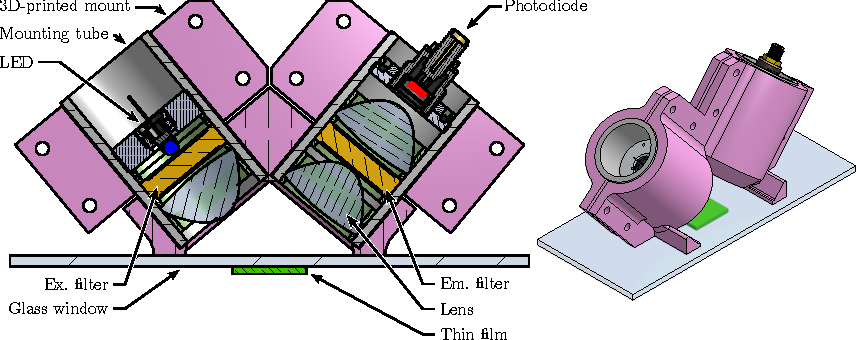
\includegraphics{1_main_matter/thin_film_figures/optoelectronics/optics_cut.pdf}
	\caption[Real-world implementation of the afore-mentioned optical parts.]{Real-world implementation of the afore-mentioned optical parts. Cut view (Left) and isometric view (Right) of the optical assembly. Note the blue and red areas on the Left side of the figure, representing the \gls{led}'s ball lens and photodiode's sensitive area, respectively. See the text for further explanations}
	\label{fig:thin_film:opto_elec:optics_cut}
\end{figure}

Briefly, Appendix~\ref{app:optical_design} details how this setup was optimised in order to maximise the amount of collected light at the photodiode. In particular, all the \gls{led} light is theoretically focused onto the thin film, and approximately 5.9\% of the re-emitted light reaches the photodiode. Using relatively pessimistic figures for the absorbance and quantum yield of the film, this results in a photocurrent in the order of 1--2~{\textmu}A for an optical \gls{led} power of 10~mW. In order to reach a voltage in the range of 100--500~mV at the photodiode amplifier's output, a transimpedance gain in the order of 10$^5$~V.A$^{-1}$ is thus needed.

\subsection{Electronic Setup}

The electronic setup used to drive the \gls{led} and amplify the photodiode's current is represented in Figure~\ref{fig:thin_film:opto_elec:elec_setup}. It was built on top of the acquisition board (NI-DAQ USB-6211, National Instruments, USA) that communicates with the computer through a \gls{usb} link. This board is further connected to the \gls{led} driver (LDP-2023, Roithner Lasertechnik, Austria) and, to the photodiode's \gls{tia} (AMP102, Thorlabs), whose gain was set to 10$^5$~V.A$^{-1}$. The LabView application, on its part, can perform \gls{fdlr} acquisitions with various excitation intensities and recording lengths---\ie{} sample count $N$. Please refer to Section \ref{sect:choos:dye_based:dlr_theory} for further details on \gls{fdlr} sensing, and Section \ref{sect:choos:phase_mes} on phase measurements.

\begin{figure}
	\centering
	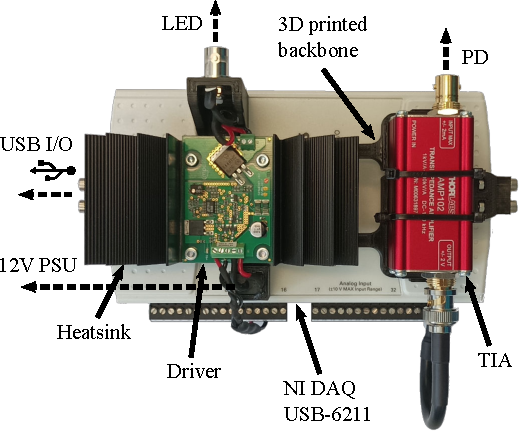
\includegraphics{1_main_matter/thin_film_figures/optoelectronics/elec_setup_comp.pdf}
	\caption[Electronic setup.]{The main active electronic components that were used, assembled together on a 3D-printed backbone. Dashed arrows represent external electrical connexions.}
	\label{fig:thin_film:opto_elec:elec_setup}
\end{figure}

\section{Thin Film Characterisation}\label{sect:thin_film:results}

Up till now, this doctoral work has:
\begin{enumerate}
	\item[--] presented the specificities of transcutaneous \gls{co2} sensing---Chapter \ref{chap:tcco2}
	\item[--] reviewed the existing \gls{co2} sensing techniques \ref{sect:choos:sensors_review}
	\item[--] chosen one \gls{co2} sensing technique according to the latter specificities: \textbf{dye-based thin film sensing}---Section \ref{sect:choos:techno_choice}
	\item[--] reviewed the chemical and optical sensing schemes associated with dye-based thin film \gls{co2} sensing---Section \ref{sect:choos:dye_based}---and chosen one of them: \textbf{dry thin films with an \gls{fdlr} sensing scheme}
	\item[--] presented the maximal theoretical accuracy reachable using this scheme---Section \ref{sect:choos:phase_mes}
	\item[--] outlined the caveats of using humidity and oxygen-sensitive luminophores and the associated workaround strategies---Section \ref{sect:thin_film:encaps}---selecting a bilayer structure for appropriate luminophore encapsulation
	\item[--] reviewed potential candidates for the luminophores and polymers used to build the said thin films---Sections \ref{sect:thin_film:select_lumino} and \ref{sect:thin_film:select_poly}---finally choosing \textbf{\gls{hpts}, \gls{rudpp}, \gls{pan}, and \gls{hpmc}} as the short- and long-lived luminophores, and \gls{rudpp}- and \gls{hpts}-encapsulating polymers, respectively
	\item[--] presented the optoelectronics that was used to probe the manufactured thin film prototypes---Section \ref{sect:thin_film:opto_elec}
\end{enumerate}
This was done with a twofold objective in mind: first, to establish a hopefully reasonable starting point for the experimentations presented below; second, to offer a comprehensive view of the motivations behind what often seems to be arbitrary choices in the literature\footnote{Without placing blame, the paper-driven research model we are accustomed to demands a conciseness that precludes the lengthy discussions found in the preceding chapters.}, as well as alternative paths for those interested in continuing this work.

The current section differs from those encountered previously in this thesis in that it adopts a more narrative style, as opposed to the conventional structure of materials and methods / results / discussion / conclusion that was used to report the experimental investigation conducted so far---\eg{} measuring haemoglobin absorption spectra, skin conductivity towards \gls{co2}, or humidity levels of occluded skin. This shift is primarily due to the still-ongoing nature of the presented research, as well as to the lack of hindsight on my part, preventing me from presenting as in-depth an analysis as I would wish to. As the reader would have surely understood by now, the optimisation of fluorescent \gls{co2}-sensing thin films is a complex matter, and the fine tuning of the numerous above-mentioned parameters is a very time-consuming process---a time I did not have. As a result, I was faced with the bitter choice of either trying to optimise a single parameter very thoroughly, or to explore superficially a few. I chose the second option, trying to do my best to at least highlight the several directions into which further work will be needed in order to achieve industry-ready, consumer-grade, \gls{fdlr} thin film-based, transcutaneous \gls{co2} sensors.

\subsection{Materials}\label{subsect:thin_film:experimental:materials}

The following chemicals were used in the next sections: \gls{rudpp} (044123.04, Thermo Fisher Scientific, USA), \gls{pan} with a mean particle size of 50µm, copolymer with 99.5m\% acrylonitrile / 0.5m\% methyl acrylate, molecular weight: 230~kg.mol$^{-1}$ (AN316010, Goodfellow, Canada), \gls{hpts} (H1529, Sigma-Aldrich, USA), \gls{hpmc} with 29m\% methoxy and 7m\% propylene oxide groups, molecular weight: 10~kg.mol$^{-1}$ (423238, Sigma Aldrich), 25\% \gls{teah} solution in methanol ($\sim$1.5~M, 86631, Sigma Aldrich), Tween 20 (P1379, Sigma Aldrich). \gls{dmf} and ethanol were of analytical grade. Wet film thicknesses were assessed with a wet film gauge, while dry film thicknesses were measured using a surface profiler (Dektak 150, Bruker, USA).

\subsection[Making Homogeneous (Not So) Thin Films]{Making Homogeneous (Not So)\protect\footnote{The term \enquote{thin film} is often used in the literature to denote film thicknesses in the nanometre range, up to 1~\textmu{}m\cite[Sect. 523-05-02]{iec62047}. In contrast, our focus is on films approximately 10~\textmu{}m thick, hence the \enquote{(Not So) Thin} heading. Of note, this 10~\textmu{}m film thickness target was set arbitrarily, based on dye-based sensing films found in the literature\cite{amao2005b, fritzsche2017, fernandezramos2019}.} Thin Films}

In order to make multilayer thin film \gls{co2} sensors, luminophore-loaded polymer thin films of the required thickness must be reproducibly manufactured, allowing the assessment of different luminophore loadings or concentrations of other chemicals---\eg{} phase transfer agent or plasticiser. Among the variety of existing polymer coating techniques---see Krebs\cite{krebs2009} and Butt\cite{butt2022}---blade coating was selected for its ability to create relatively thick---\ie{} up to tens of micrometers if needed---films while being adaptable to roll-to-roll processes for scalability. However, due to my lack of experience with this technique combined to the absence of technical expert on this matter in my laboratory, quite some time was spent to reach an acceptable reproducibility level.

\subsubsection{Polymer Solubility Assays}

Before experimenting with blade coating, solubility assays were performed to evaluate the ease of dissolution of \gls{pan} and \gls{hpmc} in \gls{dmf} and water / ethanol mixtures, respectively. A secondary objective was also to assess the viscosity and workability of the so-obtained solutions. Briefly, as some of these observations were already mentioned in Section~\ref{sect:thin_film:select_poly}, both polymers were found to be infinitely soluble in their solvents---\ie{} pure \gls{dmf} for \gls{pan}, and 1:1 or 2:1 ethanol / water mixtures for \gls{hpmc}. However, due to \textit{(i)} the formation of a gel preventing further dissolution and \textit{(ii)} the viscosity increase that prevented magnetic mechanical stirring, polymer concentrations above 15--20m\% were difficult to come by in practice.

Temperature greatly influenced the solubility of \gls{pan} in \gls{dmf}: while three hours at 80{\degree}C led to a complete dissolution of 15m\% \gls{pan}, three days at 30{\degree}C were completely insufficient, with large lumps and aggregates still present. Of note, cooling the so-obtained 80{\degree}C / 15m\% solution down to ambient temperature did not result in any \gls{pan} precipitation, allowing one to conclude that the influence of temperature is indeed on the kinetics of dissolution rather than on the solubility itself. Regarding \gls{hpmc}, no thermoreversible gelation was observed, as mentioned above---see Section~\ref{subsect:thin_film:poly_hpmc}. When using 10m\% polymer concentrations, complete dissolution was observed within 4~h using 80{\degree}C for \gls{pan} in \gls{dmf} and 55{\degree} for \gls{hpmc} in 1:1 ethanol / water mixture.

Of note, a first batch of \gls{pan} in \gls{dmf} dissolution assays completely failed, producing turbid solutions even at \gls{pan} concentration as low as 5m\%. This was attributed to the use of an old bottle of \gls{dmf} in lack of a better alternative hypothesis, since a freshly opened \gls{dmf} bottle did not exhibit this behaviour. This possible explanation is not really satisfactory, however, since \gls{dmf} is a reputedly stable compound when stored in gas-tight, opaque, containers. Nevertheless, the faulty bottle might have picked up some humidity, which may have caused hydrolysis of \gls{dmf} into dimethylamine and formic acid\cite{juillard1977}. These compounds---or the presence of water---may in turn have hampered \gls{pan} dissolution.

\subsubsection{Doctor-Blading and Screen Printing}\label{subsect:thin_film:experimental:doctor_screen}

A first series of experiments was conducted with \gls{hpmc} solutions in a 1:1 water / ethanol mixture, but what follows was also observed with \gls{pan} solutions in \gls{dmf}, and likely depends only on the mechanical properties---\ie{} viscosity, density, surface tension, \etc.---of the fluids considered. A K Control Coater (Erichsen, Germany) was used, whose basic working principle is depicted in Figure~\ref{fig:thin_film:experimental:doctor_blade}, Left. 

\begin{figure}
	\centering
	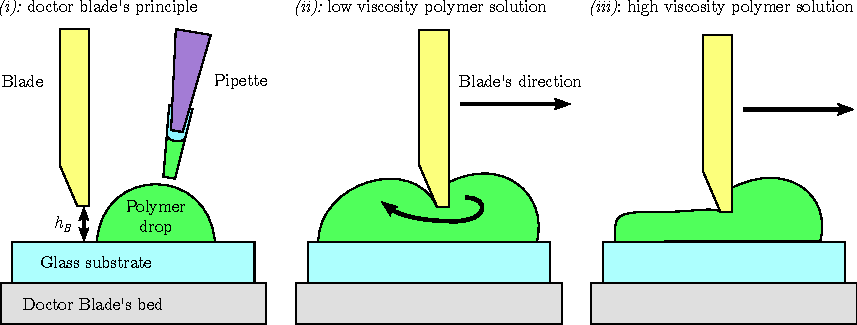
\includegraphics{1_main_matter/thin_film_figures/experimentals/doctor_blade.pdf}
	\caption[Doctor blade schematic and the bulging issue.]{Doctor blade working principle: A blade can be adjusted vertically to a height $h_B$ above the substrate. A drop of polymer is then deposited in front of the blade using a pipette \textit{(i)}. The blade then spreads the polymer drop onto the surface. However, the resulting wet film thickness is strongly dependent on the viscosity of the polymer solution. If the solution is too fluid \textit{(ii)}, it flows under the blade and bulges behind it, forming a wet film much thicker than $h_B$. Conversely, if the solution is sufficiently viscous, the bulging is minimal, and the wet film achieves the desired thickness.}
	\label{fig:thin_film:experimental:doctor_blade}
\end{figure}

At first, it was readily observed that---due to the limited amount of polymer solution that could practically be deposited at a time---$h_B$ was limited to approximately 250~\textmu{}m. Indeed, using larger substrate / blade gaps resulted in wet thin films that were thick at the beginning---\ie{} close to the blade---but which became thinner and thinner after less than 1~cm of blade travel, due to polymer depletion. Then, it was also observed that $h_B$ values in the 150--250~\textmu{}m range yielded dry film thicknesses of very similar values---0.91~\textmu{}m (SD 0.16~\textmu{}m) for $h_B=150$~\textmu{}m and 1.22~\textmu{}m (SD 0.14~\textmu{}m) for $h_B=225$~\textmu{}m when using 2m\% \gls{hpmc} solution (averages and SD computed on three measurements on three different films, 9 measurements in total for each $h_B$ value). This was ascribed to the phenomenon depicted in Figure~\ref{fig:thin_film:experimental:doctor_blade}, Centre and Right panels, \ie{} back-flow of polymer solution under the blade leading to wet thin films far thicker than $h_B$. Luckily, this behaviour disappeared when using more viscous solutions---\eg{} 10\% polymer in solution, which has a viscosity akin to that of honey, or chocolate syrup (approximately 2--10,000~cP). For instance, 10m\% \gls{pan} in \gls{dmf} yielded dry thin films of 7.87~\textmu{}m (SD 0.85~\textmu{}m) and 16.0~\textmu{}m (SD 1.3~\textmu{}m) for $h_B$ values of 100 and 200~\textmu{}m, respectively (between 7 and 12 measurements per film, on three different films, 21 and 36 measurements in total for each configuration). This 10m\% concentration was found to be a satisfactory intermediate between \textit{(i)} having a quickly dissolving solution but back-flow issues---which happened for concentrations below approximately 5m\%---and \textit{(ii)} having a solution too thick to be dissolved in a reasonable time, mixed magnetically, or practical to handle---which happened for concentrations above approximately 15m\%. For these reasons, \textbf{this 10m\% value was selected and used in the remainder of this doctoral work}, be it for \gls{pan} in \gls{hpmc} or for \gls{hpmc} in water / ethanol mixtures.

Then, a better alternative to the K Control Coater was sought: the blade must be removed for cleaning after each thin film is deposited---otherwise, gooey, partially dried polymer builds up, contaminating and scratching the next thin film---and the $h_B$ adjustment must be redone afterward using a micrometric screw and shims. This is a time-consuming process, which additionally introduces a source of variability with $h_B$ adjustment, and it was thus decided to switch to screen printing instead. To this end, a large \gls{ptfe} blade was machined, and used in combination with a framed \gls{smd} stainless steel stencil---see Appendix~\ref{app:screen_printing} for detailed drawings. \gls{ptfe} was selected because of its ease of cleaning, while framed \gls{smd} stencils were found convenient to work with. They can furthermore be ordered with arbitrary and accurate cuts to accommodate any screen printing need, while being available in various thicknesses in the 80--300~\textmu{}m range. Moving the blade was done by hand, and resulted in thin films of mean thickness 9.26~\textmu{} (SD 0.81~\textmu{}m, 6 measurements on six films, 36 measurements in total) when using a 100~\textmu{}m thick stencil and 10m\% \gls{pan} solution in \gls{dmf}. Seeing no degradation in reproducibility with using the K Control Coater---\ie{} approximately a SD of 10\% the film thickness---and being much more convenient to work with in the lab, this screen printing technique was thus adopted for the remainder of my work.

Of note, the use of coating rods---\aka{} spiral rods, coating bars, wire(-wound) bars, grooved (metering) rod, or a combination thereof---was also considered, but this trail was not explored due to a lack of time. Additionally, there was no strong incentive to try and polish the thin film fabrication technique: in case of industrial mass-production, roll-to-roll processes---fine-tuned by experts---are likely to be used. The added value of this doctoral work is thus more on the formulation of the thin film chemistry and the implementation of the sensing technique than on manufacturing thin polymer films of highly reproducible thickness.

\subsection{Successful Proof of Concept}\label{subsect:thin_film:experimental:newcas}

A first successful proof of concept was developed and presented at the NEWCAS 2024 conference\cite{dervieux2024newcas} using the afore-presented optical sensing scheme, opto-electronics, screen printing setup, and polymers / solvents / dyes combinations. The main objective of this early prototype was to validate all the components of the resulting \gls{co2}-sensing acquisition chain. Additionally, this was an ideal opportunity to also validate the theoretical considerations on the accuracy of phase measurements developed in Section~\ref{sect:choos:phase_mes}. Indeed, it has been demonstrated that, given that the phase noise of the sampling ADC can be neglected---see Equation~\hl{XX}:
\begin{equation}\label{eq:thin_film:rmse_phase_noise_gene}
	\text{RMSE} \approx \frac{1}{\sqrt{N \cdot \text{\gls{snr}}}}
\end{equation}
wherein $N$ is the number of samples, and \gls{snr} is the signal-to-noise ratio of the measured signal (see Section~\ref{sect:choos:phase_mes} for further information). Thus, by increasing either $N$ or the \gls{snr}, one should in theory be able to lower the \gls{rmse} on $\varphi_\text{mes}$ at will---a theory that I aimed to validate with the following experimentations.

\subsubsection{Material and Methods}\label{subsect:thin_film:experimental:newcas_mm}

Fluorescent thin films were fabricated using 25$\times$25~mm polished soda lime glass substrates, onto which two polymer layers were successively screen printed on top of each other. The first layer consisted of a 100~\textmu{}m-thick wet film of the following solution: 52.4~mg \gls{rudpp} and 524~mg \gls{pan} in 5~mL \gls{dmf} (1m\% of \gls{rudpp} added to a 10m\% \gls{pan} solution in \gls{dmf}). After complete solvent evaporation at room temperature, the second layer was applied, which consisted of a 100~\textmu{}m-thick wet film of the following solution: 47.0~mg \gls{hpts}, 993~mg \gls{hpmc}, 47~mg Tween 20, and 60~\textmu{}L of a 25\% \gls{teah} solution in methanol, in 10~mL of a 50:50 ethanol / distilled water mixture (1m\% of \gls{hpts} added to a 10m\% \gls{hpmc} solution in ethanol / water). The total thickness of the two stacked films was measured to be 10.9~\textmu{}m.

\subsubsection{Measurement Protocol}

Two distinct measurement sessions were performed. At first, the films were submitted to water-saturated 0, 5, 10 and back to 0\% \gls{co2} in \gls{n2} at 25{\degree}C, while measuring $\varphi_\text{mes}$ every second. A 50~kHz excitation frequency was used with a 15~mA amplitude / 20~mA offset \gls{led} driving signal, while taking $N=10$k samples per measurement at 250~kspl.s$^{-1}$.

Then, the \gls{co2} concentration was fixed to 5\% while the sample count was varied from 50 to 50k with a 15~mA fixed excitation signal amplitude in a first set of measurements. In a second phase, the amplitude of the driving signal was varied from 1 up to 24~mA with a fixed $N=10$k sample count and 24~mA offset. In these two configurations, 300 phase measurements were taken and their \gls{rmse} was computed.

The excitation frequency and sampling rate were the same in all measurements. Most importantly, the excitation frequency $f_0$, sampling frequency $f_\text{s}$, and sample count $N$, were chosen such that $N\cdot f_0/f_\text{s}$ is an integer, in order to ensure a synchronous sampling situation---see Section~\ref{sect:choos:phase_mes}. Finally, all experiments were performed under 100\% relative humidity, consistently with expected levels under occluded skin---see Section~\ref{sect:tcco2:skin_mes:rh}.

\subsubsection{Results}

\paragraph{Response to \gls{co2}}\mbox{}\\

The typical thin film response to different \gls{co2} levels may be seen in Figure~\ref{fig:thin_film:experimental:newcas_results}, Left. Initially, in pure \gls{n2}, all the \gls{hpts} is present in its strongly fluorescent anionic form. Since the fluorescence time of \gls{hpts} is only of a few nanoseconds---as opposed to that of \gls{rudpp} which is in the microsecond range---the measured phase $\varphi_\text{mes}$ is maximal, being \enquote{lifted} upwards by \gls{hpts}. On the contrary, when the percentage of \gls{co2} inside the enclosure rises, the \gls{hpts} gradually turns into its non-fluorescing protonated form. Thus, $\varphi_\text{mes}$ shifts towards lower values, being \enquote{dragged} downward by the long fluorescence time of \gls{rudpp}.

\begin{figure}
	\centering
	\includegraphics{1_main_matter/thin_film_figures/experimentals/tikz/out/newcas_results.pdf}
	\caption[Phase response of the fluorescent thin film upon exposure to different \gls{co2} levels, and evolution of the phase \gls{rmse}.]{\textbf{Left:} phase response of the fluorescent thin film (in black) upon exposure to different \gls{co2} levels (in blue). The red, dash-dotted, vertical lines correspond to the times at which the gaseous mixture in the enclosure was changed from pure \gls{n2} to 5\% \gls{co2}, 10\% \gls{co2}, and pure \gls{n2} again. \textbf{Right:} \gls{rmse} of the phase measurements. Each data point is computed from 300 phase measurements. The associated (log-log) linear regressions are least-square fitted ($R^2 \geq 0.99$).}
	\label{fig:thin_film:experimental:newcas_results}
\end{figure}

Unfortunately, while Figure~\ref{fig:thin_film:experimental:newcas_results}, Left, indicates no major time lag between changes in \gls{co2} levels and the associated phase shifts of the thin film, measuring the response time of the latter proved challenging due to the slow response time of the enclosure. In other words, it takes a considerable amount of time for the system to reach a specific \gls{co2} level. Addressing this limitation is currently under investigation to shorten the equilibrium time of the measurement setup, thus enabling the characterization of the thin film's response time. Still, making the approximation that \textit{(i)} the sensor is a first-order system, and that \textit{(ii)} it responds to a ramp of \gls{co2}---which holds relatively true at the beginning of the \gls{co2} exponential response where it is almost linear---leads to a response time estimation of about 47~s, which is on par with the existing literature of thin film dye-based \gls{co2} sensing---see Section~\ref{subsect:choos:review:dye_based} and references therein.

\paragraph{Theoretical Results Validation}\mbox{}\\

Figure~\ref{fig:thin_film:experimental:newcas_results}, Right, presents on a logarithmic scale the experimental validation of former theoretical results describing the decline of the phase measurement RMSE with an increase in $N$ or \gls{snr}---see Section~\ref{sect:choos:phase_mes}\todo{Ajouter ref à l'équation exacte quand l'article de phase sera finalisé.}. In this case, Equation~\ref{eq:thin_film:rmse_phase_noise_gene} becomes:
\begin{equation}\label{eq:thin_film:log_first}
	\log(\text{\gls{rmse}}) = -\frac{1}{2}\cdot \log(N) - \frac{1}{2}\log(\text{\gls{snr}})
\end{equation}
Since $\text{\gls{snr}} = \frac{A^2}{2\cdot \sigma_x^2}$, wherein $A$ is the amplitude of the excitation signal and $\sigma_x$ the variance of the additive Gaussian noise added, Equation~\ref{eq:thin_film:log_first} further becomes:
\begin{equation}\label{eq:thin_film:compact_rmse_A}
	\log(\text{\gls{rmse}}) = -\frac{1}{2}\cdot \log(N) - \log(A) + \log(\sqrt{2}\cdot \sigma_x)
\end{equation}

This equation explains the slopes of the two linear regressions performed in Figure~\ref{fig:thin_film:experimental:newcas_results}, Right. Indeed, when $N$ is varied with a constant illumination intensity (Figure~\ref{fig:thin_film:experimental:newcas_results}, Right, in red), the observed slope of -0.46 is close to the theoretical value of $-\sfrac{1}{2}$. Similarly, when the \gls{led} intensity is varied while keeping a constant sample count (Figure~\ref{fig:thin_film:experimental:newcas_results}, Right, in blue), the observed slope of -0.95 is close to the theoretical value of $-1$, which is expected since the optical power $A$ of an \gls{led} is directly proportional to its driving current.

Those two results thus validate the theory presented in Section~\ref{sect:choos:phase_mes}, and allow for a better comprehension of the reachable accuracy in an \gls{fdlr} sensing scheme. In particular, they show that even with a moderate number of samples and a relatively low intensity---\ie{} 10k samples (40~ms at 250kspl/s) and 15~mA---an \gls{rmse} below 0.03{\degree} can be reached. This \gls{rmse} would in turn translate into errors in \gls{co2} concentration estimation of roughly 0.05\% ($\approx$0.4~mmHg), according to the results presented in Figure~\ref{fig:thin_film:experimental:newcas_results}, Left, which may be acceptable for \gls{ptco2} monitoring in clinical practice\cite{conway2018}.

\subsubsection{Conclusion}

This first proof of concept gives promising clues for the use of an \gls{fdlr} sensing scheme for accurate \gls{co2} sensing in general, and hopefully to \gls{ptco2} monitoring applications in particular. Of note, the results presented in Figure~\ref{fig:thin_film:experimental:newcas_results} are in good agreement with existing literature on the topic of thin film, fluorescence-based, \gls{co2} sensing\cite{borisov2011}, as well as with the theoretical considerations on the accuracy of \gls{fdlr} measurements presented in Section~\ref{sect:choos:phase_mes}. In particular, these results indicate that a shorter acquisition with a higher emission power---\ie{} decreasing $N$ and increasing $A$---may be desirable from an \gls{rmse} and power consumption point of view. This paves the way for power consumption analyses similar to that recently presented by Ebrahimi \etal{} in the case of \gls{ppg} sensors\cite{ebrahimi2023}, but for \gls{dlr}-, fluorescent-based \gls{co2} sensors.

The obtained fluorescent thin film exhibited a clear correlation between its phase shift and the surrounding \gls{co2} concentration, even if its response time could unfortunately not be measured accurately, a limitation that should be addressed in future works. Experimental validation of theoretical findings regarding the decline of $\varphi_\text{mes}$ \gls{rmse} with increased sample count or signal-to-noise ratio also demonstrated that---even with a modest number of samples and limited illumination power---an accuracy below 0.03{\degree} on $\varphi_\text{mes}$ may be reached. This value in turn leads to \gls{pco2} estimation accuracy well below medical expectations.

Despite these encouraging results, two significant issues remain: a strong influence of humidity on the intensity of \gls{hpts} fluorescence was observed, and some amount of photobleaching also affected both \gls{hpts} and \gls{rudpp}.

\subsection{Humidity Influence}\label{sect:thin_film:experimental:humid}

\subsubsection{The Issue}

Glass slides were prepared as described in Section~\ref{subsect:thin_film:experimental:newcas_mm}, but with only one of the two luminescent thin films---\ie{} with only a film of \gls{hpts} in \gls{hpmc} or with only a film of \gls{rudpp} in \gls{pan}. While no humidity influence was observed for the \gls{rudpp} / \gls{pan} films, \gls{hpts} / \gls{hpmc} films were on the contrary exceedingly sensitive to it, as illustrated in Figure~\ref{fig:thin_film:experimental:humidity_influence}, Left. Two compatible hypotheses may explain this observation, and are discussed below.

\begin{figure}
	\centering
	\includegraphics{1_main_matter/thin_film_figures/experimentals/tikz/out/humidity_influence.pdf}
	\caption[Humidity influence on \gls{hpts} thin films fluorescence, and comparison with the water uptake of other polymers.]{\textbf{Left:} humidity influence on the fluorescence intensity of \gls{hpts} thin films measured at 27{\degree} in pure \gls{n2}. The breaks in the curve observed at 90 and 93\% are due to a lack of data on the 90--93\% \gls{rh} range, a linear interpolation was thus used to fill the resulting gap. The intensity was normalised with respect to its value at 50\% \gls{rh}. \textbf{Right:} water uptake of different compounds as a function of \gls{rh}. Data sources: polyacrylic acid sodium salt (PAA-Na), \gls{peg}, and silica data come from Thijs \etal{}\cite{thijs2007} and were measured at 30{\degree}C, while \gls{hpmc} data are those of 100cp Affinisol from Patel \etal{}\cite{patel2022_part2}, and were measured at 25{\degree}C.}
	\label{fig:thin_film:experimental:humidity_influence}
\end{figure}

\subsubsection{First Hypothesis}

\textbf{($\mathcal{H}_1$): there is not enough hydration water in the \gls{hpmc} matrix at ambient humidity levels}---\ie{} in the 40--60\% \gls{rh} range---and only by reaching very high \gls{rh} values can sufficient amounts of water be available for \gls{hpts} to fluoresce strongly\footnote{Dry \gls{hpts} crystals do not fluoresce strongly, as opposed to their solution in water. When films dry out, they turn from a bright fluorescent yellow-green to a pale non-fluorescent yellow. Personal observations.}. This first hypothesis is comforted by the fact that water uptake curves for \gls{hpmc} follow the same exponential aspect as in Figure~\ref{fig:thin_film:experimental:humidity_influence}, Left. This exponential aspect is indeed shared by a variety of hygroscopic polymers, as can be seen in Figure~\ref{fig:thin_film:experimental:humidity_influence}, Right---let us ignore silica data, which are discussed below---but also in the works of Thijs \etal{}\cite{thijs2007}, Patel \etal{}\cite{patel2022_part1, patel2022_part2, patel2023_part3} and Yang \etal{}\cite{yang2020capsule}, to cite a few.

If ($\mathcal{H}_1$) is true, this humidity sensitivity issue may be mitigated by choosing a more hygroscopic polymer than \gls{hpmc}, such as gelatin, pullulan\cite{yang2020capsule}, hydroxypropyl cellulose\cite{patel2022_part2}, poly\-vinyl\-pyrrolidone\cite{patel2023_part3}, PAA-Na\cite{thijs2007}, \gls{peg}, sorbitol, or carboxymethyl cellulose sodium salt\cite{callahan1982}, for instance. Additionally, adding more significant amounts of some hygroscopic plasticisers---\eg{} glycerol or \gls{peg}---might also be beneficial to increase \gls{hpmc} water uptake\cite{malik2022}. Indeed, the quantity of Tween 20 that we added was mainly a guesstimate based on the work of Fernandez-Ramos \etal{}\cite{fernandezramos2018}, and amounts to about 4m\% of the dry film. By contrast, other authors---not attempting at manufacturing \gls{co2} sensing films, but rather studying the water uptake properties of polymer / plasticisers pairs---used plasticiser contents in the 20--50m\% range\cite{suyatma2005, zeppa2009, khwaldia2013, malik2022}, \ie{} ten times more than we did.

Alternatively, no amount of uptaken water might be \emph{enough} to completely eliminate the humidity dependence of the fluorescence intensity of \gls{hpts}-containing thin films. In other words, the issue may lie not in the water uptake of \gls{hpmc} being too low, but in its increase with humidity---\ie{} the slope of \gls{hpmc}'s water uptake isotherm---being too large. In this latter case, it might be a better choice to move to a not-so-hygroscopic material that has an almost flat water uptake isotherm, such as silica---see Figure~\ref{fig:thin_film:experimental:humidity_influence}, Right. Indeed, it has almost the same water uptake across the full 60--90\% \gls{rh} range. A film-forming polymer with this kind of behaviour might thus be an interesting alternative to \gls{hpmc}.

Finally, since it has been suggested that hydration water might be bound to the phase transfer agent---\gls{tmah}, in our case---rather than to the polymer itself, as mentioned in Section~\ref{subsect:thin_film:breath_poly:poly_select}, maybe solely increasing the \gls{tmah} concentration could reduce humidity cross-sensitivity. In the same line of thought, several authors also mentioned increasing the phase transfer agent concentration for stability purposes\cite{neurauter1999, ge2003, cajlakovic2006, aguayolopez2014}. This \mfrin{}trail thus deserves particular attention for upcoming developments on the presented work.

\subsubsection{Second Hypothesis}

\textbf{($\mathcal{H}_2$): water uptake changes the optical properties of the \gls{hpmc} thin films}. Indeed, swelling usually accompanies water uptake in hygroscopic polymers to some extent\cite{grossutti2020}, which may  change how light propagates throughout thin films. Water uptake can also influence the refractive index\cite{watanabe1998} or the transparency of polymer layers\cite{gulsen2006}. In the particular case of \gls{hpmc}, Trezza \etal{}\cite{trezza2000} reported a decrease in gloss and an increase in whiteness index with increasing humidity levels, while Laksmana \etal{}\cite{laksmana2008} reported a significant swelling of \gls{hpmc} with increasing \gls{rh} values. Both these phenomena may in turn influence light propagation inside the \gls{hpmc} thin films, and thus their resulting fluorescence intensity. For instance, a strong haziness of the films may induce strong scattering within the films and increase the resulting fluorescence signal, in a similar way to when \ce{TiO2} particles are added\cite{dansby2010}.

However, this second hypothesis does not seem extremely likely given the magnitudes of the above-mentioned phenomena, and was mainly mentioned here for the sake of not neglecting any potential research avenue. Of note, while there exists an extensive literature\footnote{See \eg{} Gao \etal{}\cite{gao1996} which is a good stereotype of the said literature.} on the swelling mechanisms of (potentially doped with numerous types of plasticisers, nanoparticles, pigments, and the like) \gls{hpmc} \emph{matrices}---\ie{} \gls{hpmc} powder pressed into tablets---almost no studies were available on the swelling and change in optical properties of \gls{hpmc}-based \emph{thin films}.

\subsubsection{Is This Even a Problem?}

At first glance, the fact that a 5--10\% \gls{rh} increase can more than double the \gls{hpts} fluorescence intensity when the latter is entrapped in \gls{hpmc} thin films---as shown in Figure~\ref{fig:thin_film:experimental:humidity_influence}, Left---may seem devastating for the future of dye-based \gls{co2} sensing as presented in the second half of this doctoral work. However, things may in fact not be as desperate as they appear: as discussed in Section~\ref{sect:tcco2:skin_mes:rh}, occluded skin is likely to be humidity-saturated, meaning a constant 100\% \gls{rh} value. If this holds true, humidity cross-sensitivity will not be an issue in real-world transcutaneous applications. Yet, this cross-sensitivity remains an issue for the in-lab thin film characterisation---and formulation optimisation---processes. Indeed, achieving humidity levels above approximately 95\% proved to be exceedingly difficult in practice: if any single part of the gas piping after the humidification stage---or any part of the enclosure containing the film under test---is below the gas temperature, condensation occurs at the culprit cold spot, thus lowering the humidity content of the gas below 100\%. Of note, while adding heating elements inside the enclosure and a heated sleeve around gas pipes mitigates the issue, it remained unfeasible to reach humidity levels in the 95--100\% range. Alas, this latter range is that of highest humidity cross-sensitivity---Figure~\ref{fig:thin_film:experimental:humidity_influence}, Left. This makes the difficulty of reaching humidity saturation particularly troublesome in practice. \mfrin{}Therefore, eliminating the humidity cross-sensitivity of \gls{hpts} thin films still seems essential, and should be the subject of future research. Additionally, 100\% \gls{rh} does not translate into the same water chemical activity depending on the temperature\cite{huang2018}. Thus, if it is this activity that impacts \gls{hpts} fluorescence and not the \gls{rh} level \textit{per se}, even saturated humidity conditions would be particularly cross-sensitive towards temperature.

Of note, while the above-mentioned difficulty in reaching very high humidity levels holds for the main gas mixing and equilibration setup that was used for the majority of my experiments---\ie{} a modified \hl{[Ref. appareil]} setup which achieves accurate regulation of both humidity and temperature ($\pm$\hl{0.1}{\degree}C\todo{à vérifier}, $\pm$\hl{0.5}\% \gls{rh})---a secondary enclosure was built using means at hand. The latter could not achieve as good temperature and humidity regulation accuracies ($\pm$0.5{\degree}C, $\pm$1.5\% \gls{rh}), but made it possible to reach $\leq$99\% \gls{rh}, at the cost of condensation inside the enclosure. This secondary enclosure was used for the \gls{hpts} photobleaching measurements presented below.

\subsection{Photobleaching and Quenching}\label{subsect:thin_film:experimental:pbl}

As mentioned in Section~\ref{subsect:thin_film:encaps:photobleaching}, both photobleaching and \gls{o2} luminescence quenching were expected to be major issues, especially concerning \gls{rudpp} phosphorescence. Thus, investigations were conducted on both luminophores in the presence and absence of oxygen.

\subsubsection{\texorpdfstring{\gls{hpts}}{HPTS} Photobleaching}\label{subsect:thin_film:experimental:pbl:hpts}

Starting with \gls{hpts}, the photobleaching of thin films entrapping it in \gls{hpmc} is shown in Figure~\ref{fig:thin_film:experimental:hpts_photobleaching}. The film composition is identical to that described in Section~\ref{subsect:thin_film:experimental:newcas_mm}, and the films were exposed to $\geq$99\% \gls{rh} and 25.4$\pm$0.2{\degree}C for over one hour. Probing was achieved using the same above-presented \gls{fdlr} setup, but looking at the modulus of the \gls{dft} of the measured signal, instead of its phase. Optical probing was performed each second, using a 50~kHz modulated sine wave, having a 15~mA amplitude and 20~mA offset, recording 10~k samples at 250~kspl.s$^{-1}$---\ie{} 40~ms probing pulses. Between the pulses, the blue \gls{led} was lit up with a 40~mA current to speed up photobleaching. To give an idea of the scale, this translates into an illumination power of about 180~W.m$^{-2}$\footnote{Value computed for a 1~cm spot diameter, assuming no losses in the illumination block, and using Thorlabs LED450L's efficiency and intensity / voltage characteristics.}.

\begin{figure}
	\centering
	\includegraphics{1_main_matter/thin_film_figures/experimentals/tikz/out/hpts_photobleaching.pdf}
	\caption[\gls{hpts} photobleaching.]{Temporal evolution of the fluorescence intensity of \gls{hpts} thin films under heavy illumination, normalised with respect to time origin. Although photobleaching is not necessarily a first-order reaction\cite{demchenko2020}, an exponential fit led to a slightly higher $R^2$ than a linear one in this particular case ($R^2 \approx 0.995$). Using a linear model led to a photobleaching rate of 11.3\%.h$^{-1}$.}
	\label{fig:thin_film:experimental:hpts_photobleaching}
\end{figure}

It appears that \gls{hpts} is quite sensitive to photobleaching, consistently with the above-mentioned observation of Nairn \etal{}\cite{nairn2015}. A first-order time constant of approximately 8.37~h was observed, corresponding to a loss in fluorescence intensity of 11.7\%.h$^{-1}$. However, this may not pose a problem for practical \gls{ptco2} sensing applications: as presented in Section~\ref{subsect:thin_film:experimental:newcas}, using a number of samples $N=10$~k and a 24~mA offset / 15~mA amplitude probing signal results in an already very satisfying accuracy. These conditions translate into a signal of 24~mA average value (9--39~mA peak to peak) and 40~ms duration. If the final \gls{ptco2} sensor takes one measurement per minute during two weeks of patch wearing\footnote{This duration was chosen based on the practical lifetime of transcutaneous blood glucose monitors---\eg{} Freestyle Libre (Abbott, USA).}, this results in 806~s of total illumination. Using a linear dependency of photobleaching on light intensity---which is likely to be a worst case\footnote{Photobleaching is often non-linearly dependent on illumination power, and higher power levels lead to significantly faster photobleaching\cite{widengren1996, diaspro2006}.}---the resulting \gls{hpts} fluorescence intensity decrease would be of only 1.85\%. Still, this phenomenon could be further minimised by two different means.

At first, the measurement conditions could be fine-tuned towards lower intensities: keeping a 15~mA amplitude, the offset could be lowered down to 15~mA without loss in accuracy, resulting in a 15~mA average value (0--30~mA peak to peak). Additionally, both the amplitude and length of the signal could be decreased, leading in a predictable---using Equation~\ref{eq:thin_film:compact_rmse_A}---loss in accuracy at the expense of much less photobleaching. In particular, if the \gls{hpts} photobleaching phenomenon---and especially its (non-)linearity towards illumination power---were accurately known, it would be possible to choose between increasing or decreasing the sample number and illumination power while minimising photobleaching. \mfrin{}Further research on the \gls{hpts} photobleaching should thus be conducted if its occurrence proves to be an issue in practice.

Second, as mentioned in Section~\ref{subsect:thin_film:encaps:photobleaching}, anti-fading agents can be added to reduce the photobleaching of luminophores. In the particular case of \gls{hpts}, \gls{dabco}---\aka{} \gls{teda}---has been reported by a number of authors to greatly reduce photobleaching, resulting in extremely photostable sensing films\cite{goicoechea2007, duong2019}. Alas, time was running short to try and add some \gls{dabco} to my \gls{hpts} thin films. This second trail therefore remains a \mfrin{}future path to explore to further reduce \gls{hpts} photobleaching.

\subsubsection{\texorpdfstring{\gls{rudpp}}{Rudpp} Photobleaching and Quenching}\label{subsect:thin_film:experimental:pbl:rudpp}

\gls{rudpp} photobleaching was assessed using the same probing scheme as \gls{hpts}---\ie{} one short probing pulse per second with heavy illumination in between---in eight configurations, which correspond to two modalities of three different parameters ($2^3=8$).
\begin{enumerate}
	\item Two different \textbf{film formulations} were tested, changing the \gls{rudpp} encapsulation polymer: using \gls{pan} (10~mL \gls{dmf}, 1.05~g \gls{pan}, 17.5~mg \gls{rudpp}), and using \gls{hpmc} (10~mL ethanol, 5~mL water, 1.29~g \gls{hpmc}, 21.5~mg \gls{rudpp}\footnote{Contrary to \gls{hpts} / \gls{hpmc} films, the ethanol / water ratio was increased to 2:1 due to the poor solubility of \gls{rudpp} in water which led to incomplete dissolution otherwise.}). The idea was to validate our polymer choice by comparing a highly \gls{o2}-impermeable polymer (\gls{pan}) with a highly \gls{o2}-permeable one (\gls{hpmc}). It was expected that photobleaching should be less pronounced in \gls{pan} than in \gls{hpmc}, especially in ambient air ($\mathcal{E}_1$).
	\item Two different \textbf{film drying methods} were evaluated: drying the films in ambient air, or in vacuum for 10~min. Vacuum drying was expected to remove the small air bubbles that may otherwise be present inside the films, and thus decrease the presence of \gls{o2} within them. Photobleaching was thus expected to be less marked in vacuum dried films, ($\mathcal{E}_2$).
	\item Two different \textbf{atmospheres} were tested, both at 25{\degree}C: dry \gls{n2}, and ambient air (38\% RH). Due to the harmful role of \gls{o2} in photobleaching, it was expected that dry \gls{n2} would lead to less photobleaching than ambient air, ($\mathcal{E}_3$).
\end{enumerate}
The resulting reductions in phosphorescence intensity are illustrated in Figure~\ref{fig:thin_film:experimental:rudpp_pbl_boxplot}.

\begin{figure}
	\centering
	\includegraphics{1_main_matter/thin_film_figures/experimentals/tikz/out/rudpp_pbl_boxplot.pdf}
	\caption[Box-plot of \gls{rudpp} photobleaching in different conditions.]{\gls{rudpp} photobleaching expressed as relative intensity decrease under different conditions. Each box-plot corresponds to six different films whose photobleaching was measured during 3000~s, and whiskers extend at most to 1.5 times the interquartile range. Median values are indicated in parentheses in the x-axis ticks' labelling.}
	\label{fig:thin_film:experimental:rudpp_pbl_boxplot}
\end{figure}

At first, it is reassuring to note that \gls{rudpp} photobleaching is relatively low for all the conditions tested. With median values in the 1--8\%.h$^{-1}$ range\footnote{No exponential fit was performed for \gls{rudpp} due to the unexpected shapes of the photobleaching curves---see Figure~\ref{fig:thin_film:experimental:rudpp_pbl_temporal}. Thus, those photobleaching rates were measured on 3000~s acquisitions and scaled to get a \enquote{per hour} value.}, this translates into a real-world phosphorescence intensity decrease in the 0.2--1.8\% range over two weeks of measurements, taking one measurement per minute. It also appears that photobleaching is lower in \gls{n2} than in ambient air, as expected ($\mathcal{E}_3$). However, the other results reported in Figure~\ref{fig:thin_film:experimental:rudpp_pbl_boxplot} are quite surprising, deceiving some of the above-presented expectations. Indeed, vacuum drying the films does not seem to have any major impact on photobleaching, apart perhaps from slightly reducing the dispersion of the measurements\footnote{This would require more tests to confirm, although a Bartlett test comparing the variances of \gls{n2} and ambient air populations (N=24 in each population) led to a p-value below 10$^{-4}$ (normality was tested using Shapiro-Wilk test, after $x\mapsto \sqrt{x}$ transformation).}, so ($\mathcal{E}_2$) is not verified. In the meantime, while \gls{pan} encapsulation does reduce photobleaching in \gls{n2} as compared to \gls{hpmc} this is no longer the case in ambient air, whereas the opposite behaviour was expected---\ie{} no major difference in \gls{n2} but a major photobleaching decrease in ambient air, ($\mathcal{E}_1$). More shockingly, air dried \gls{hpmc} exhibits a negative value in ambient air!

\begin{figure}
	\centering
	\includegraphics{1_main_matter/thin_film_figures/experimentals/tikz/out/rudpp_pbl_temporal.pdf}
	\caption[Temporal evolution of \gls{rudpp} photobleaching.]{Temporal evolution of \gls{rudpp} photobleaching. Films were air dried and photo\-bleached in ambient air.}
	\label{fig:thin_film:experimental:rudpp_pbl_temporal}
\end{figure}

To better understand what happened, some additional measurements were taken using much longer recording durations (26~000~s / 7.2~h). Corresponding representative temporal plots can be observed in Figure~\ref{fig:thin_film:experimental:rudpp_pbl_temporal}: while \gls{pan} films exhibit an exponential decrease from early on, \gls{hpmc} films first exhibit some strange behaviour before settling to reach a steady-state photobleaching rate after some three hours. The reason for this is still unclear at the moment, with no plausible candidate hypotheses at hand. Maybe some impurities initially present in \gls{hpmc} can promote \gls{rudpp} phosphorescence before being photobleached, but this seems quite unlikely, and the mystery remains. Besides this first anomaly, observing Figure~\ref{fig:thin_film:experimental:rudpp_pbl_temporal} in the 3--7~h range still gives a much higher photobleaching rate for \gls{pan} than for \gls{hpmc} ($\sim$2.4 \textit{vs} 0.7\%.h$^{-1}$). This is against all odds, and in contradiction with the afore-mentioned existing literature on photobleaching, \gls{o2} permeability, and encapsulation---see Sections~\ref{sect:thin_film:encaps} and \ref{subsect:thin_film:rudpp_poly}. Again, the reason for this is still unclear. One \mfrin{}possible trail to follow would be to study more thoroughly the photobleaching of \gls{rudpp} in a variety of media---\ie{} in several polymers and solvents---to try and identify a pattern or degradation pathway for this photobleaching.

Lastly, \gls{rudpp} phosphorescence quenching was also assessed by observing the phase shifts of \gls{rudpp} phosphorescence signals, which are represented in Figure~\ref{fig:thin_film:experimental:rudpp_quenching_boxplot}. Again, it seems that vacuum drying reduces the variability of measurements, especially in the case of \gls{pan} films. However, contrary to the photobleaching case, the encapsulating effect of \gls{pan} seems to be effective, since $\varphi_\text{mes}$ changes of less than 0.5{\degree} for \gls{pan} films between \gls{n2} and ambient air, whereas it shifts by almost 3{\degree} for \gls{hpmc} in the meantime. That being said, the reader should take these last results with a \emph{shaker} of salt, as it was observed that phase measurements tended to be influenced by the fluorescence intensity as well. This is a flaw of the photodiode's \gls{tia}, which appears to have led to phase measurement errors in the $\pm$1{\degree} range\footnote{This error should be thought of as an offset---\ie{} a constant value added to $\varphi_\text{mes}$---being dependent on both the amplitude and offset of the signal that the \gls{tia} sees.}. This latter observation triggered the development of a double-stage, op-amp based, low-noise and high-gain \gls{tia} to try and mitigate this issue. However, this amplifier has not been tested yet, and thus remains beyond the scope of this thesis.

\begin{figure}
	\centering
	\includegraphics{1_main_matter/thin_film_figures/experimentals/tikz/out/rudpp_quenching_boxplot.pdf}
	\caption[Box-plot of \gls{rudpp} phosphorescence quenching in different conditions.]{Phase shifts of \gls{pan} and \gls{hpmc} thin films containing \gls{rudpp} under various conditions. Each box-plot corresponds to six different films, and whiskers extend at most to 1.5 times the interquartile range. Median values are indicated in parentheses in the x-axis ticks' labelling. Corresponding decay times assuming a first order decay phenomenon are given on the right axis ($\tau_\textit{R}=-\frac{\tan(\varphi_\text{mes})}{2\cdot\pi\cdot f}$, $f=50$~kHz). Be cautious that the right axis scale is thus non-linear.}
	\label{fig:thin_film:experimental:rudpp_quenching_boxplot}
\end{figure}

\section{Conclusion}\label{sect:thin_film:conclusion}

This chapter begins---Section~\ref{sect:thin_film:encaps}---with the presentation of two photochemical mechanisms that make luminescence measurement practically challenging: namely photobleaching and quenching. Those phenomena tend to affect particularly long-lived luminophores---\ie{} phosphors---and call for some kind of mitigation strategy. To this end, it was decided to select an \gls{o2} impermeable polymer for the phosphor that ended up being used, and a multilayer thin film architecture.

A second part---Sections~\ref{sect:thin_film:select_lumino} and \ref{sect:thin_film:select_poly}---focuses on the selection of appropriate chemicals, based on the different criteria that the previous chapter established: fluorescence lifetime, permeability, availability, cost, ease of implementation, stability, \etc{}. This benchmarking work led to the selection of two dye / polymer pairs: \gls{rudpp} in \gls{pan}, and \gls{hpts} in \gls{hpmc}.

A third part---Section~\ref{sect:thin_film:opto_elec}---briefly presents the electronics that were used for practical \gls{dlr} measurements, while the detailed design study associated with the optical design and electronics dimensioning is relegated to Appendix~\ref{app:optical_design}.

Finally, a fourth part---Section~\ref{sect:thin_film:results}---concentrates on an experimental validation of the theory presented and choices made throughout all the above sections and chapters. While an initial proof of concept yielded encouraging results, many research questions remain open, particularly regarding dye photobleaching and humidity influence on \gls{hpts}-containing thin films.

These observations conclude the present chapter, which is the last to report the contributions of this doctoral work and the penultimate chapter of this thesis. Unlike the previous chapters, this one is much more experimental in nature, and since time was running short, several drastic, arbitrary choices had to be made. Similarly, several questions remain unanswered. Fortunately, to ensure the reader is not left wanting more, a final chapter explores the future research prospects envisioned to continue this work.
